\documentclass{article}
\usepackage{graphicx}
\usepackage{amsmath}
\usepackage{amsfonts}
\usepackage{bookmark}
\usepackage{booktabs}
\usepackage{exercises}
\graphicspath{ {./images/8.6} }
\usepackage{indentfirst}
\usepackage{amsthm}
\usepackage{yhmath}
\usepackage{geometry}
\usepackage{placeins}
\usepackage{csquotes}
\usepackage{pgfplots}
\newcommand*{\oldneg}{\mathord{\sim}}
\newcommand\showdiv[1]{\overline{\smash{)}#1}}
\newcommand\Mydiv[1]{%
\smash{\raise.3ex\hbox{$\big)$}}\mkern-8mu
        \overline{\enspace\strut#1}}
\setlength{\tabcolsep}{5pt}
\theoremstyle{definition}
\newtheorem{definition}{Definition}

\setlength{\parindent}{.5in}
\setlength{\parskip}{12pt}
\renewcommand{\arraystretch}{2}
\geometry{margin=1in}
\newcommand{\?}{\stackrel{?}{=}}
\pgfplotsset{width=7cm,compat=1.18}\usepgfplotslibrary{statistics}

\title{8.6 Answers}
\begin{document}
\maketitle

\section*{1}
They are called conic sections as they are all formed when a plane intersects a double-napped cone.

\section*{2}
A general second-degree equation is defined to be of the form $Ax^2+Bxy+Cy^2+Dx+Ey+F=0$. The discriminant is 
$B^2-AC$. If $B^2-AC<0$ and $B=0$ and $A=C$, then the conic represented by the equation is a circle. If $B^2-4AC<0$ but either $B\ne 0$ or $A\ne C$, then 
the conic represented by the equation is an ellipse. If $B^2-4AC=0$, then the conic represented by the equation is a parabola. If $B^2-4AC>0$, then the conic 
represented by the equation is a hyperbola.

\section*{8}
This is a circle centered at $(5,-1)$ with a radius of $\sqrt{64}=8$:\newline
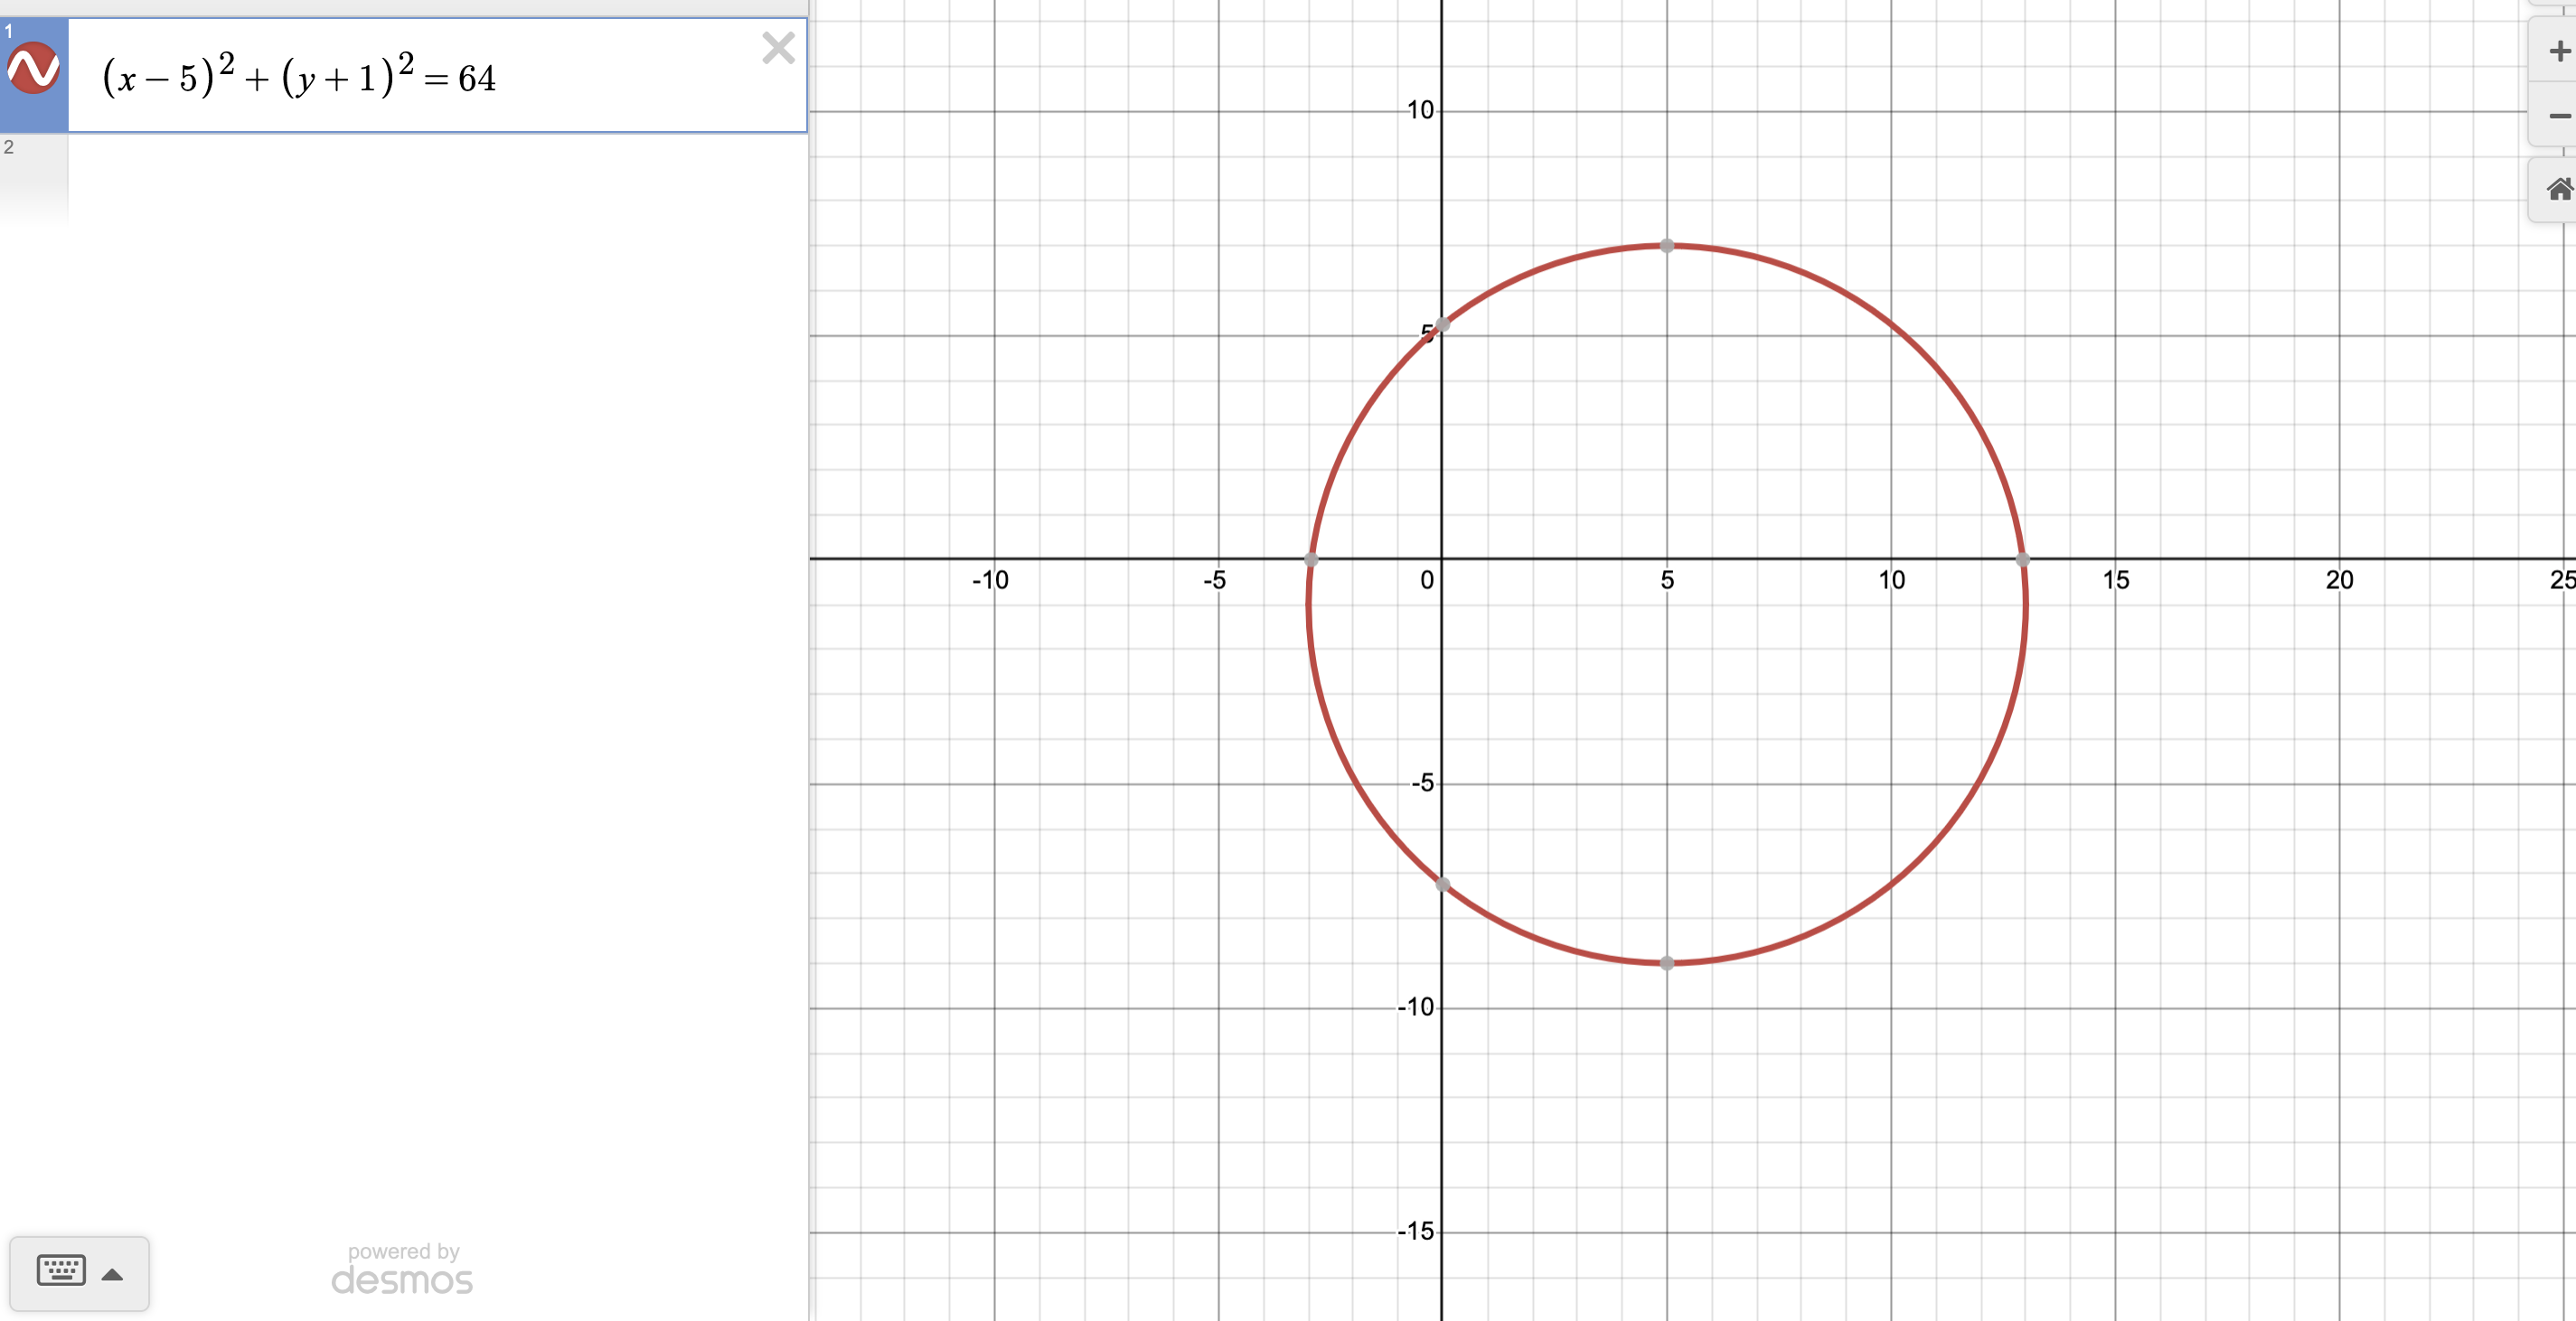
\includegraphics[width = 4in]{8}

\section*{9}
This is a parabola with a vertex of $(-6,1)$. Thus it has an axis of symmetry of $y=1$. Then we also know that $p=\frac{4}{4}=1$, and thus the focus is 
$(-5,1)$ and the directrix is $x=-7$:\newline
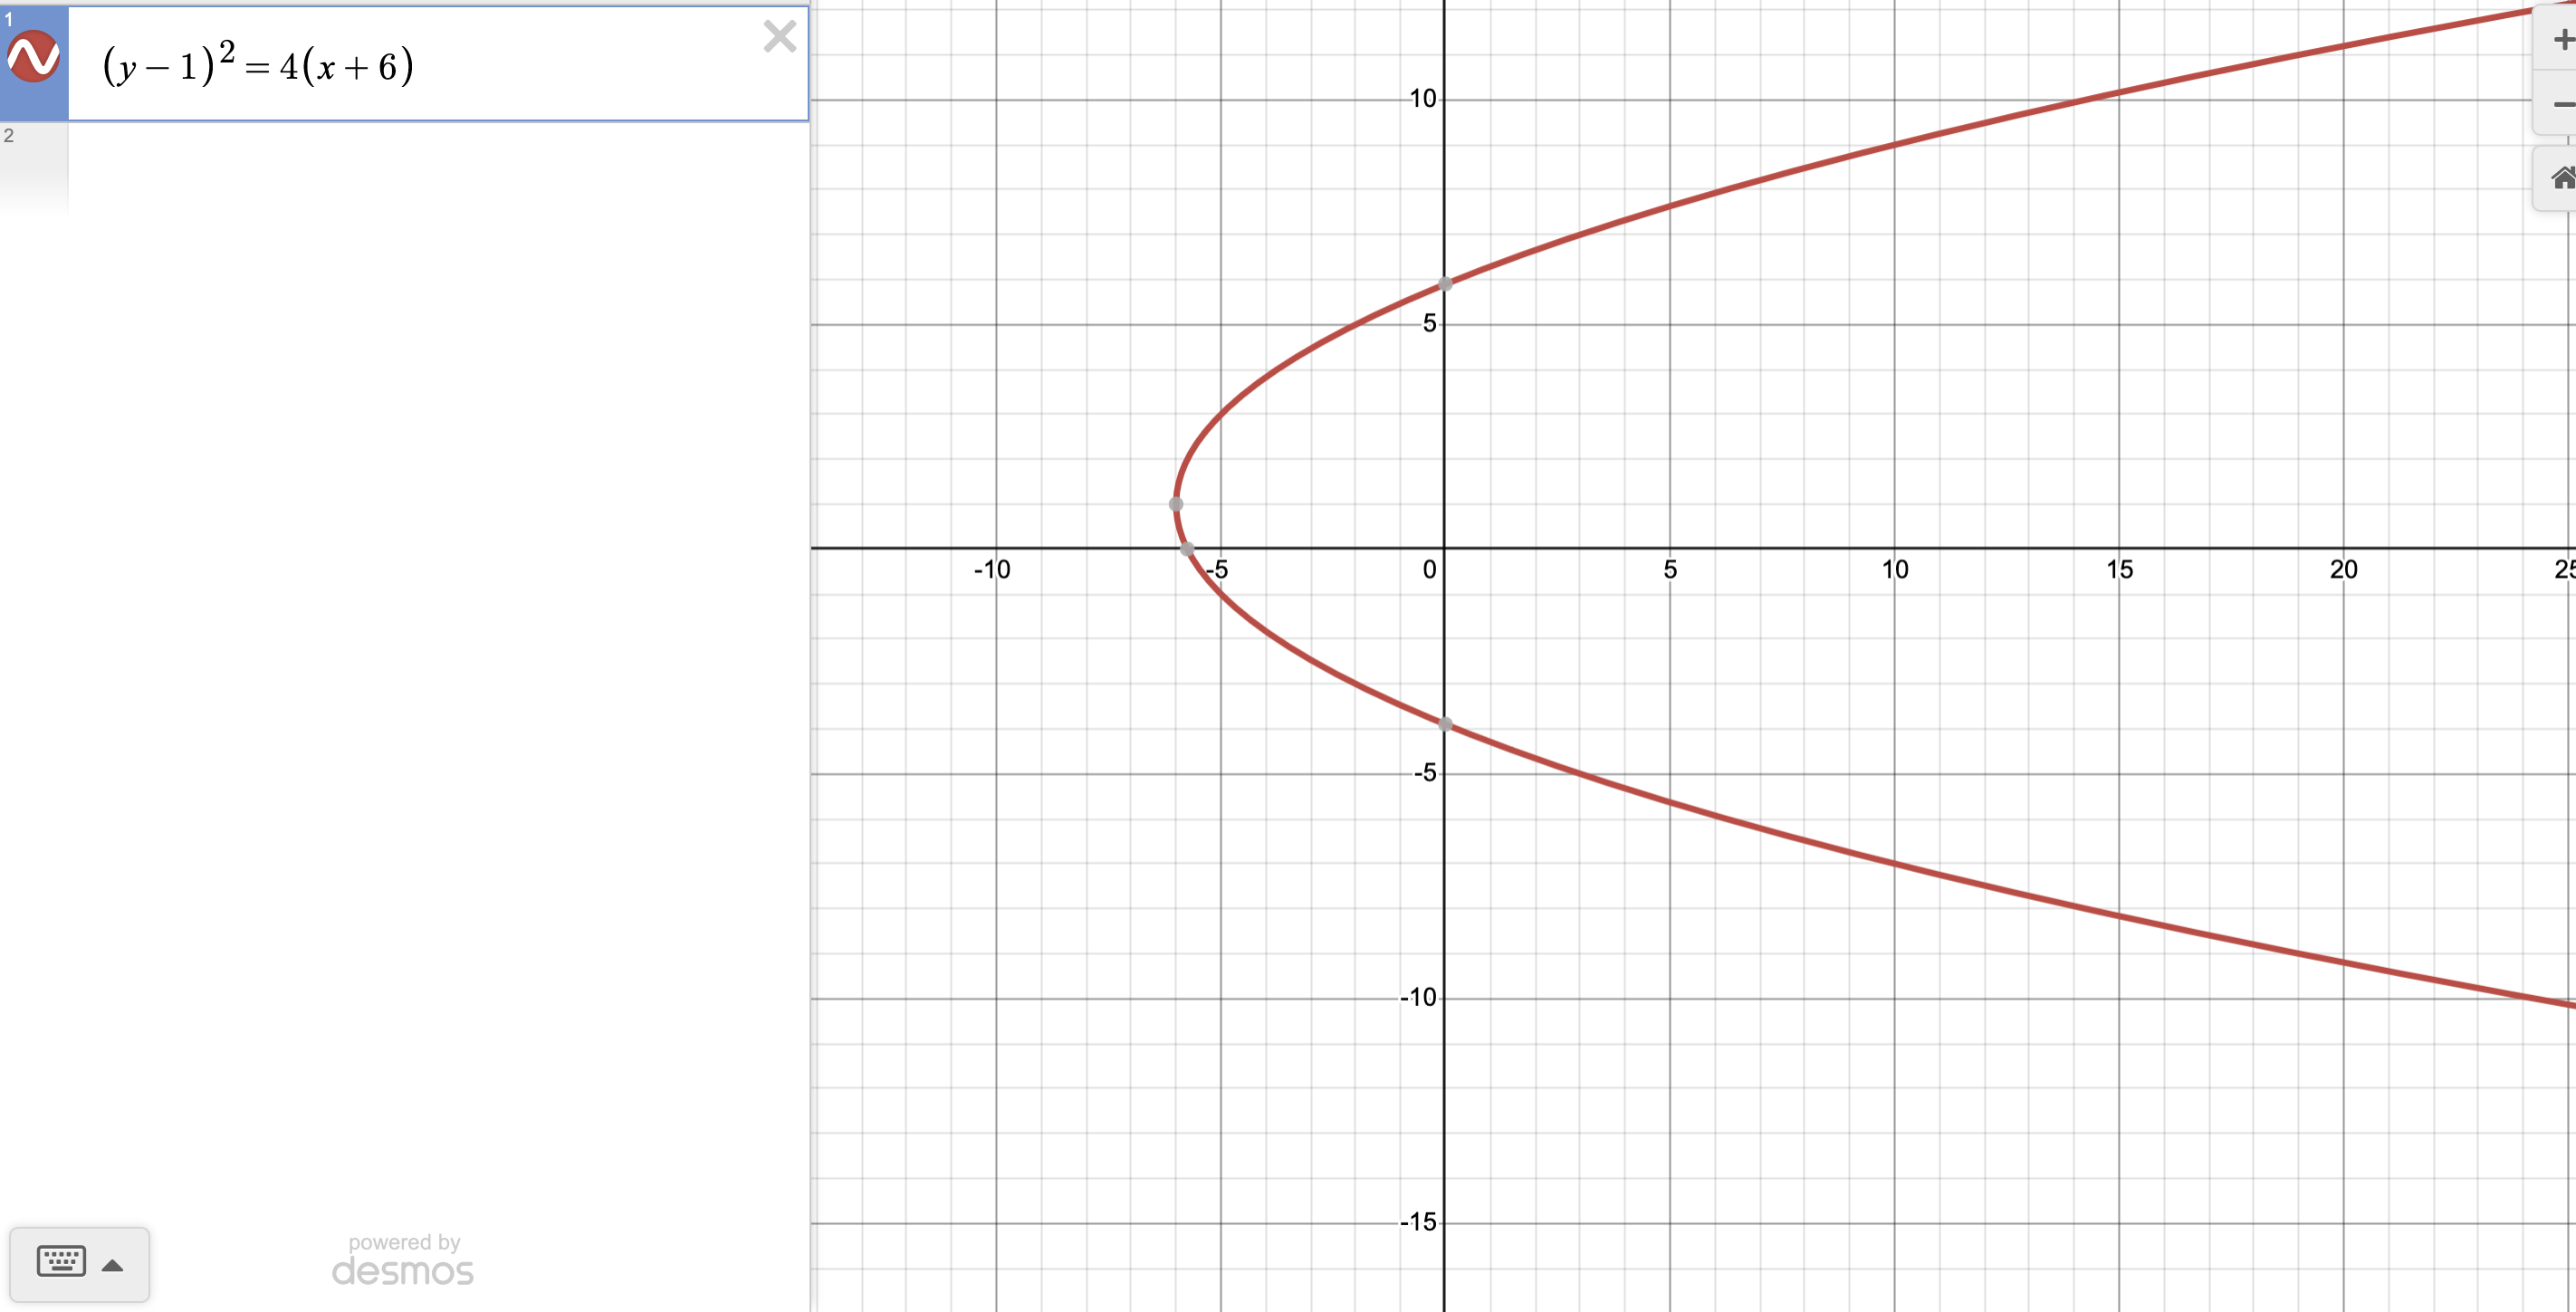
\includegraphics[width = 4in]{9}

\section*{10}
This is an ellipse centered at $(0,2)$, with $a=\sqrt{25}=5$ and $b=\sqrt{4}=2$. Also, the major axis is horizontal. Hence the vertices are 
$(0\pm 5,2)$ and the co-vertices are $(0,2\pm 2)$. Then we can find $c$:
\[ c^2=5^2+2^2 \] \[ c=\sqrt{29} \] meaning the foci lie $\sqrt{29}$ units away from the center, that is, the foci are:
$(1\pm\sqrt{29},2)$:\newline
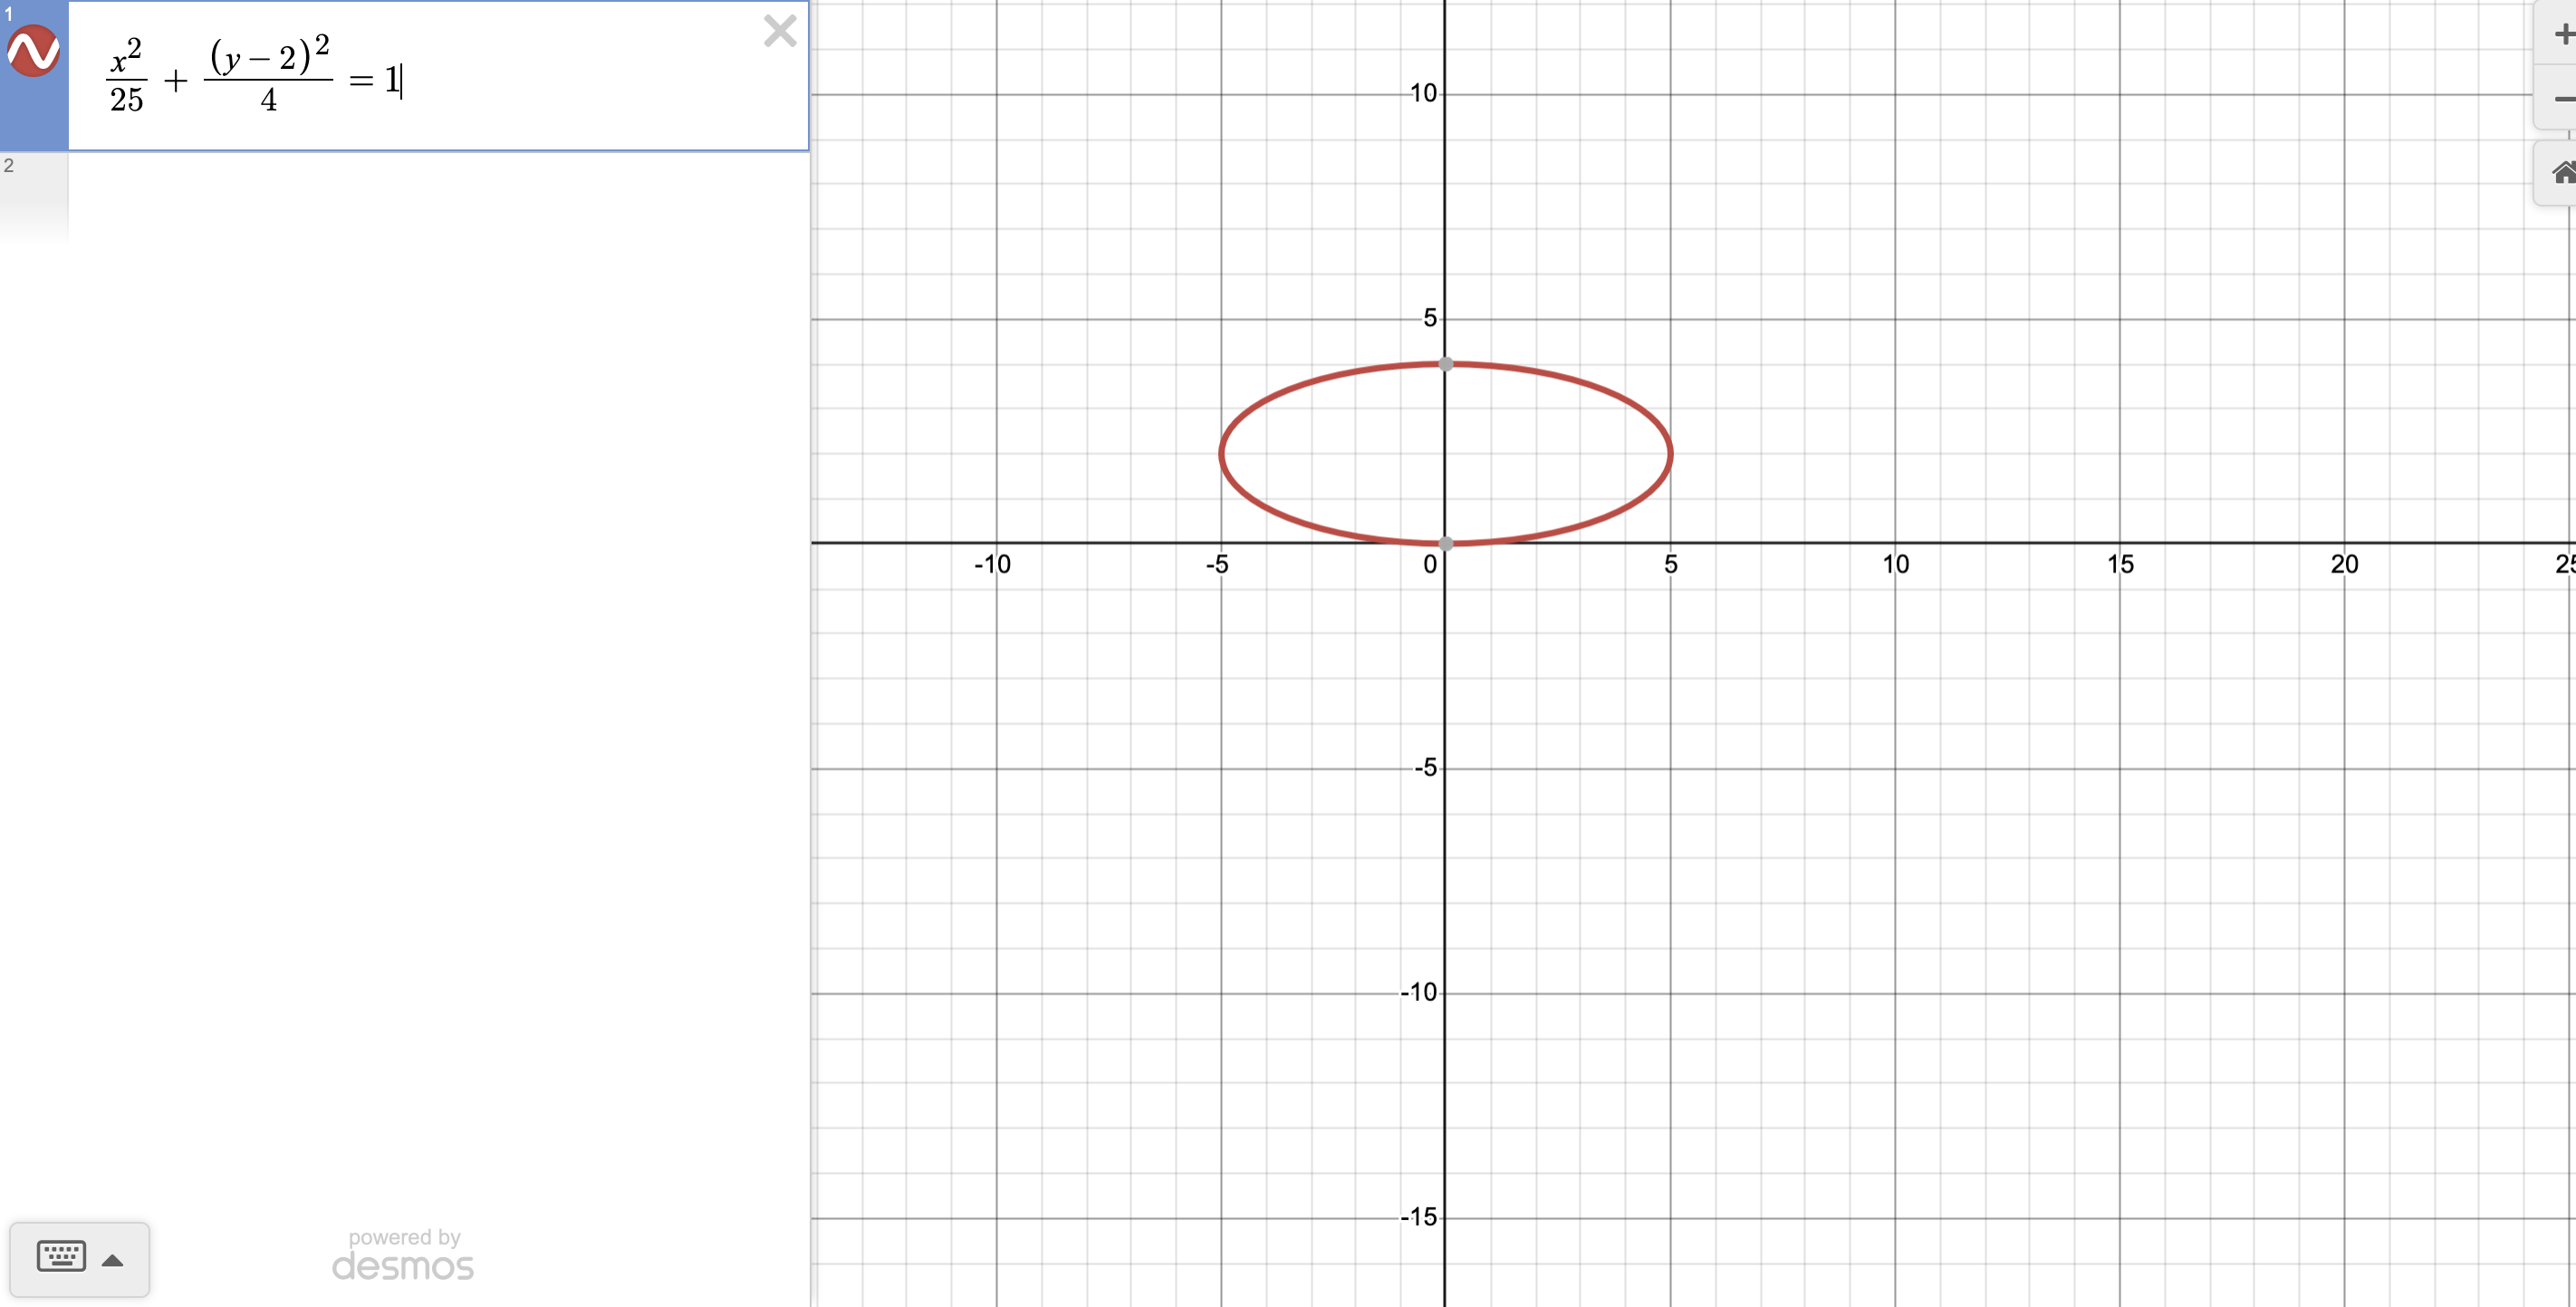
\includegraphics[width = 4in]{10}

\section*{11}
This is a hyperbola centered at $(-3,4)$, with $a=\sqrt{9}=3$ and $b=\sqrt{16}=4$. The transverse axis is horizontal. Thus we know that the vertices are 
$(-3\pm 3,4)$ and
\[ c^2=9+16 \] \[ c=5 \] meaning the foci are $(-3\pm 5,4)$. We also know that the asymptotes are $y=\pm\frac{3}{4}$:\newline
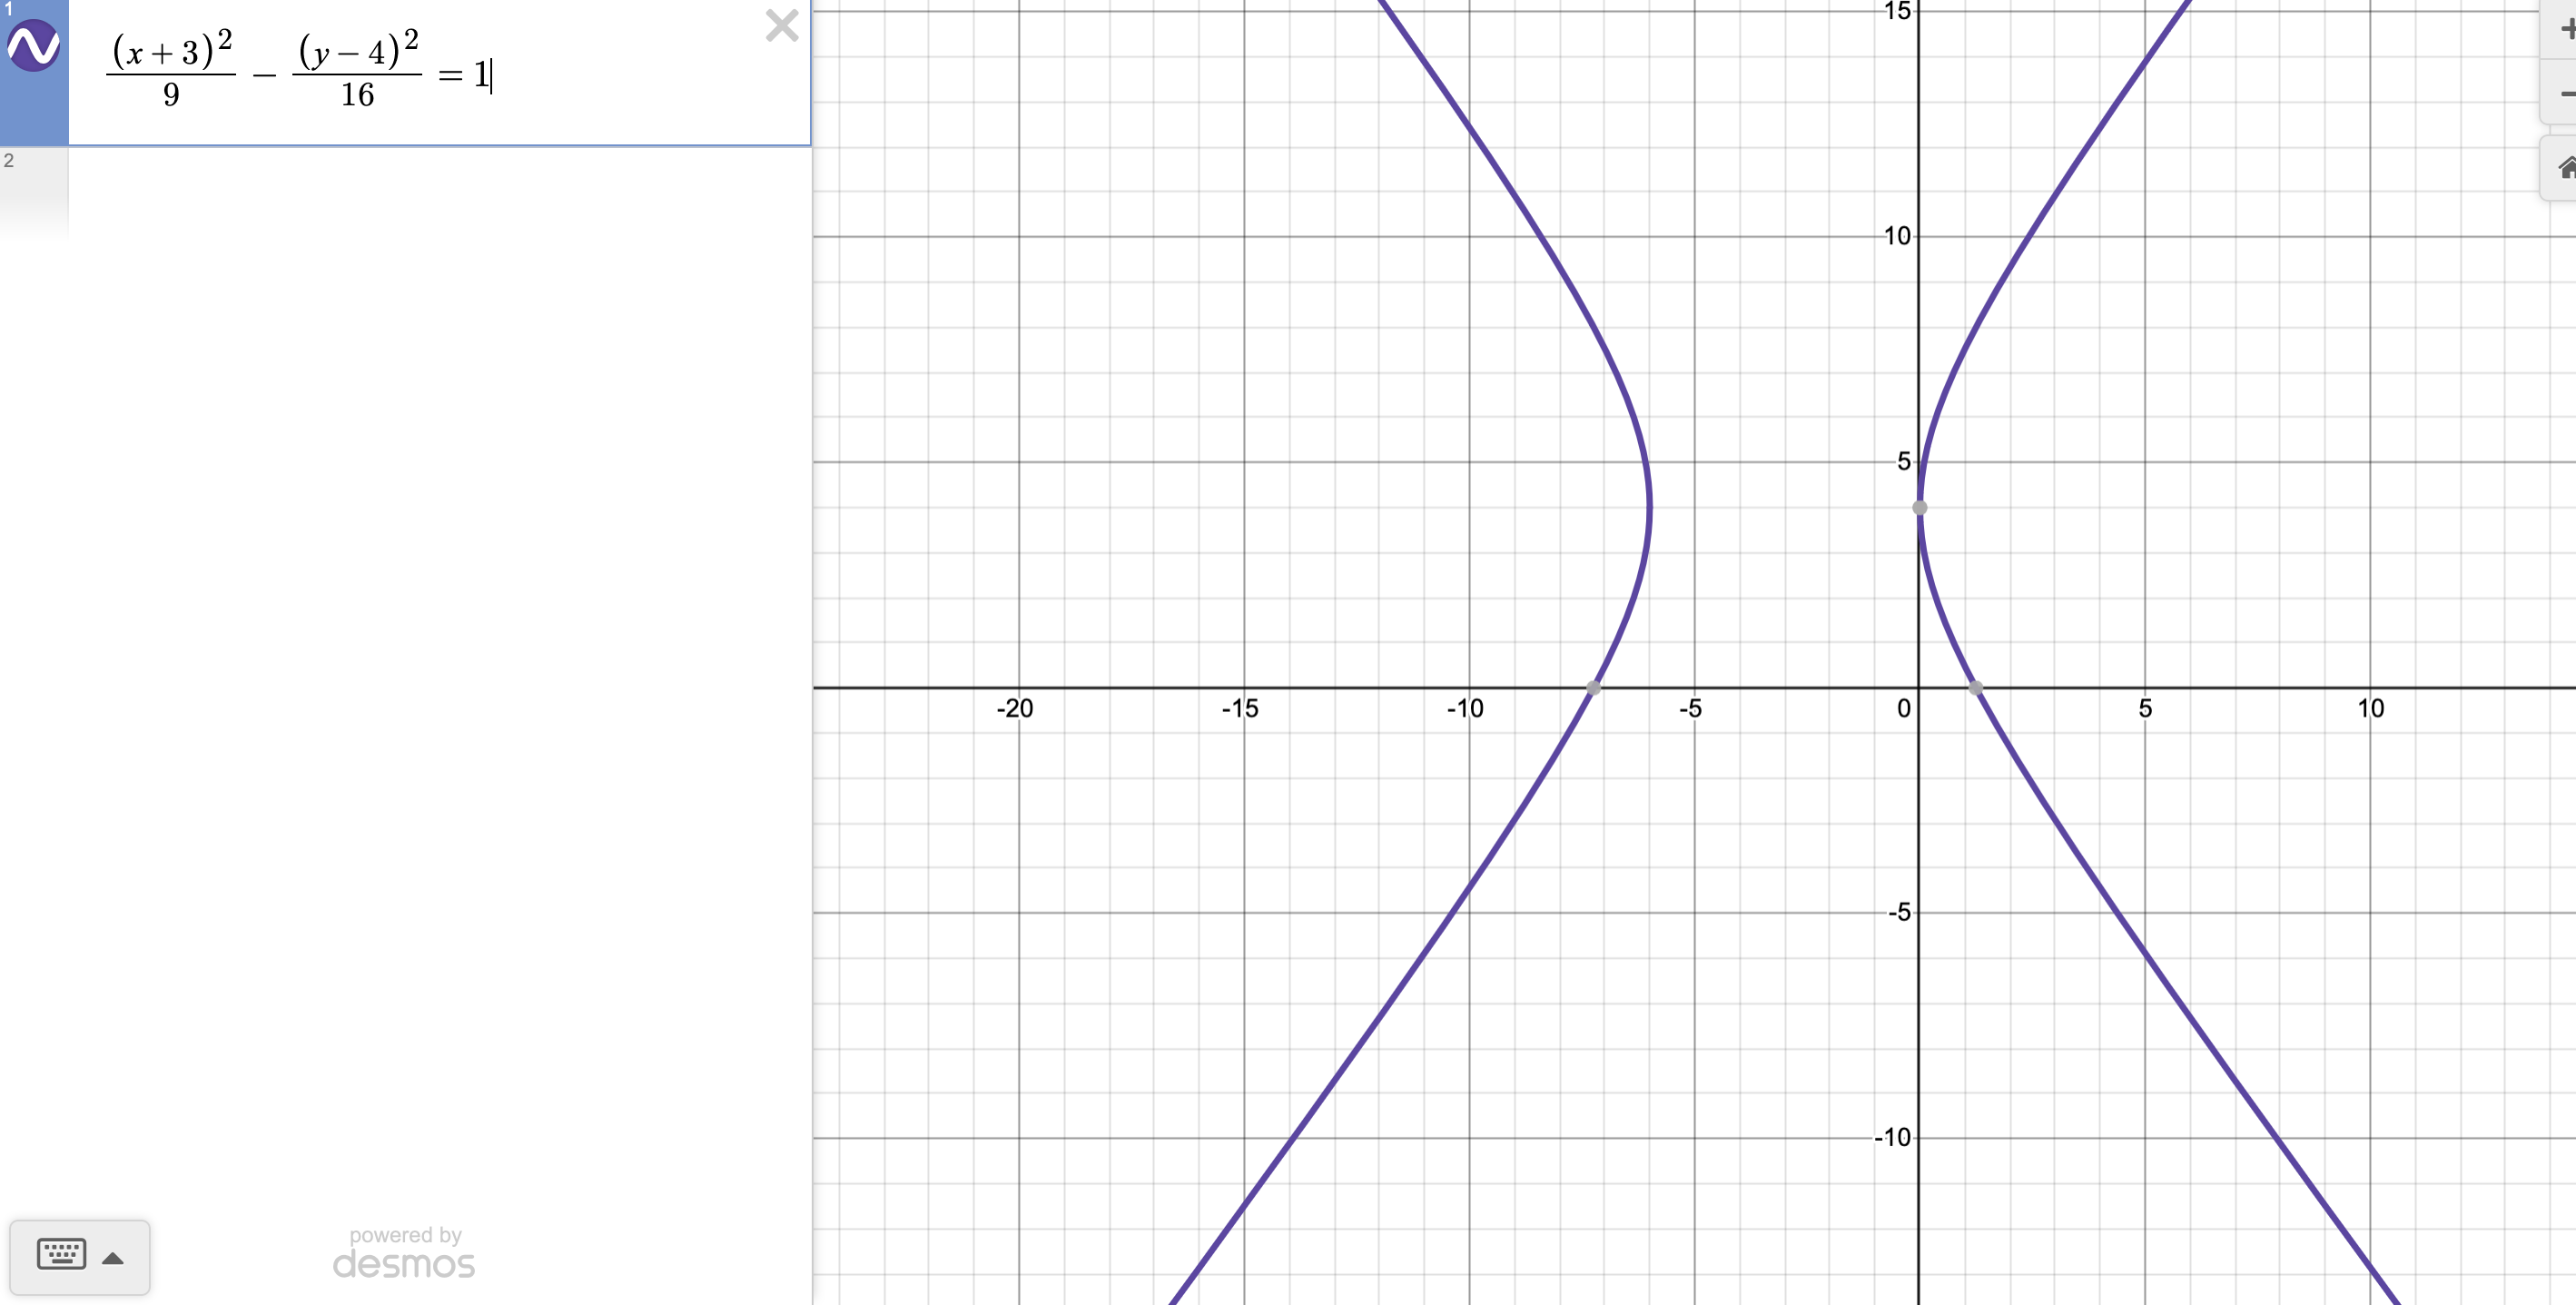
\includegraphics[width = 4in]{11}

\section*{12}
We are given an ellipse centered at $(4,1)$ with a horizontal major axis, $a=\sqrt{16}=4$, and $b=\sqrt{4}=2$. Thus the co-vertices are 
$(4,1\pm 2)$, that is, $(4,3)$ and $(4,-1)$. Thus the answer is C.

\section*{13}
We are given a circle centered at $(-5,1)$ and with a radius of 6, meaning it's equation is $(x+5)^2+(y-1)^2=36$.

\section*{14}
We are given a circle centered at $(9,-1)$ and with a radius of 2, meaning it's equation is $(x-9)^2+(y+1)^2=4$.

\section*{15}
We are given a parabola with a vertex at $(-4,-3)$ and a focus at $(1,-3)$. Thus the parabola is of the form (as it has a horizontal axis):
$(y+3)^2=4p(x+4)$. But we know that $p=|1+4|=5$, meaning the equation is $(y+3)^2+20(x+4)$.

\section*{16}
We are given a parabola with a vertex at $(5,3)$ and a directrix $y=6$. Thus $p=3-6=-3$ and the axis of symmetry is vertical. Thus the equation is
$(x-5)^2=-12(y-3)$.

\section*{17}
We are given an ellipse with vertices at $(-3,4)$ and $(5,4)$ and foci at $(-1,4)$ and $(3,4)$. Thus the major axis is horizontal. 
We know that the center is halfway between the vertices. 
Hence the center is $(\frac{-3+5}{2},4)=(1,4)$. This means that $a=4$ and $c=2$. Thus:
\[ 2^2=4^2-b^2 \] \[ b^2=12 \] meaning the equation for the ellipse is $\frac{x^2}{16}+\frac{y^2}{12}=1$.

\section*{18}
We are given an ellipse with vertices at $(-2,1)$ and $(-2,9)$ and co-vertices at $(-4,5)$ and $(0,5)$. Thus the major axis is vertical. We know that 
the center is halfway between the vertices. Hence the center is $(-2,\frac{1+9}{2})=(-2,5)$. Thus, $a=4$ and $b=2$, meaning an equation for the ellipse is
$\frac{(x+2)^2}{4}+\frac{(y-5)^2}{16}=1$.

\section*{19}
We are given a hyperbola with vertices at $(6,-3)$ and $(6,1)$ and foci at $(6,-6)$ and $(6,4)$. Thus the transverse axis is vertical. We know that the center is 
halfway between the vertices. Hence the center is $(6,\frac{-3+1}{2})=(6,-1)$. Thus $a=2$ and $c=5$, meaning:
\[ 25=4+b^2 \] \[ b^2=21 \] meaning an equation for the hyperbola is $\frac{(y+1)^2}{4}-\frac{(x-6)^2}{21}=1$.

\section*{20}
We are given a hyperbola with vertices at $(1,7)$ and $(7,7)$ and foci at $(-1,7)$ and $(9,7)$. Thus the transverse axis is horizontal. We know that the center is 
halfway between the vertices. Hence the center is $(\frac{1+7}{2},7)=(4,7)$, meaning $a=3$ and $c=5$, and thus:
\[ 25=9+b^2 \] \[ b^2=16 \] meaning an equation for the hyperbola is $\frac{(x-4)^2}{9}-\frac{(y-7)^2}{16}=1$.

\section*{21}
We are given an ellipse with vertices at $(-7,3)$ and $(3,3)$ and co-vertices at $(-2,6)$ and $(-2,0)$. It is correct that the axis is horizontal. The correct center 
is also given. The second line is also correct, finding the correct values for $a$ and $b$. However, the last line is incorrect, as the center is $(-2,3)$, not 
$(2,-3)$. The answer probably mistakes the standard form of ellipses to be $\frac{(x+h)^2}{a^2}+\frac{(y+k)^2}{b^2}=1$, but, when the axis is horizontal, it is actually 
$\frac{(x-h)^2}{a^2}+\frac{(y-k)^2}{b^2}$. Thus the correct answer is $\frac{(x+2)^2}{25}+\frac{(y-3)^2}{9}=1$.

\section*{22}
We are given an ellipse with a center of $(-5,2)$. The lines of symmetry of an ellipse are the vertical and horizontal lines through the center. Thus the lines of 
symmetry are $x=-5$ and $y=2$. 

\section*{24}
We are given a hyperbola centered at $(1,2)$. The lines of symmetry of the hyperbola are the vertical and horizontal lines through the center. Thus the lines of 
symmetry are $x=1$ and $y=2$.

\section*{26}
We are given a parabola with a vertex of $(-3,1)$. Because it is the term with $x$ that is being squared in the equation, we know that the axis of symmetry is the 
vertical line passing through the vertex, that is, $x=-3$. 

\section*{27}
We are given a circle centered at $(-2,-1)$. Thus the lines of symmetry for the circle are any lines which pass through the center of the circle.

\section*{32}
We know that $9=1,B=0$ and $C=4$. Thus the discriminant is $0-4(4)(9)<0$, and because $A\ne C$, the conic represented by this equation is an ellipse.

\section*{33}
We know that $A=1,B=0$ and $C=0$. Thus the discriminant is $0-0=0$, meaning the conic represented by this equation is a parabola.

\section*{34}
We know that $A=1,B=0$ and $C=1$. Thus the discriminant is $0-4=-4<0$, and because $B=0$ and $A=C$, the conic represented by this equation is a circle.

\section*{35}
We know that $A=8,B=0$ and $C=-9$. Thus the discriminant is $0-4(8)(-9)=288>0$, meaning the conic represented by this equation is a hyperbola.

\section*{36}
We know that $A=4,B=0$ and $C=1$. Thus the discriminant is $0-4(4)=-16<0$, and because $A\ne C$, the conic represented by this equation is an ellipse. Thus the 
answer is B.

\section*{41}
We know that $A=9,B=0$ and $C=4$, meaning the discriminant is $0-4(4)(9)<0$, and because $A\ne C$, the conic represented by this equation is an ellipse. We need to 
complete the square twice to turn the equation into one of an ellipse:
\[ 9x^2+4y^2-36x-24y+36=0 \] \[ 9(x^2-4x)+4(y^2-6)+36=0 \]
\[ 9(x^2-4x+4)+4(y^2-6+9)+36=36+36 \]
\[ 9(x-2)^2+4(y-3)^2=36 \]
\[ \frac{(x-2)^2}{4}+\frac{(y-3)^2}{9}=1 \]
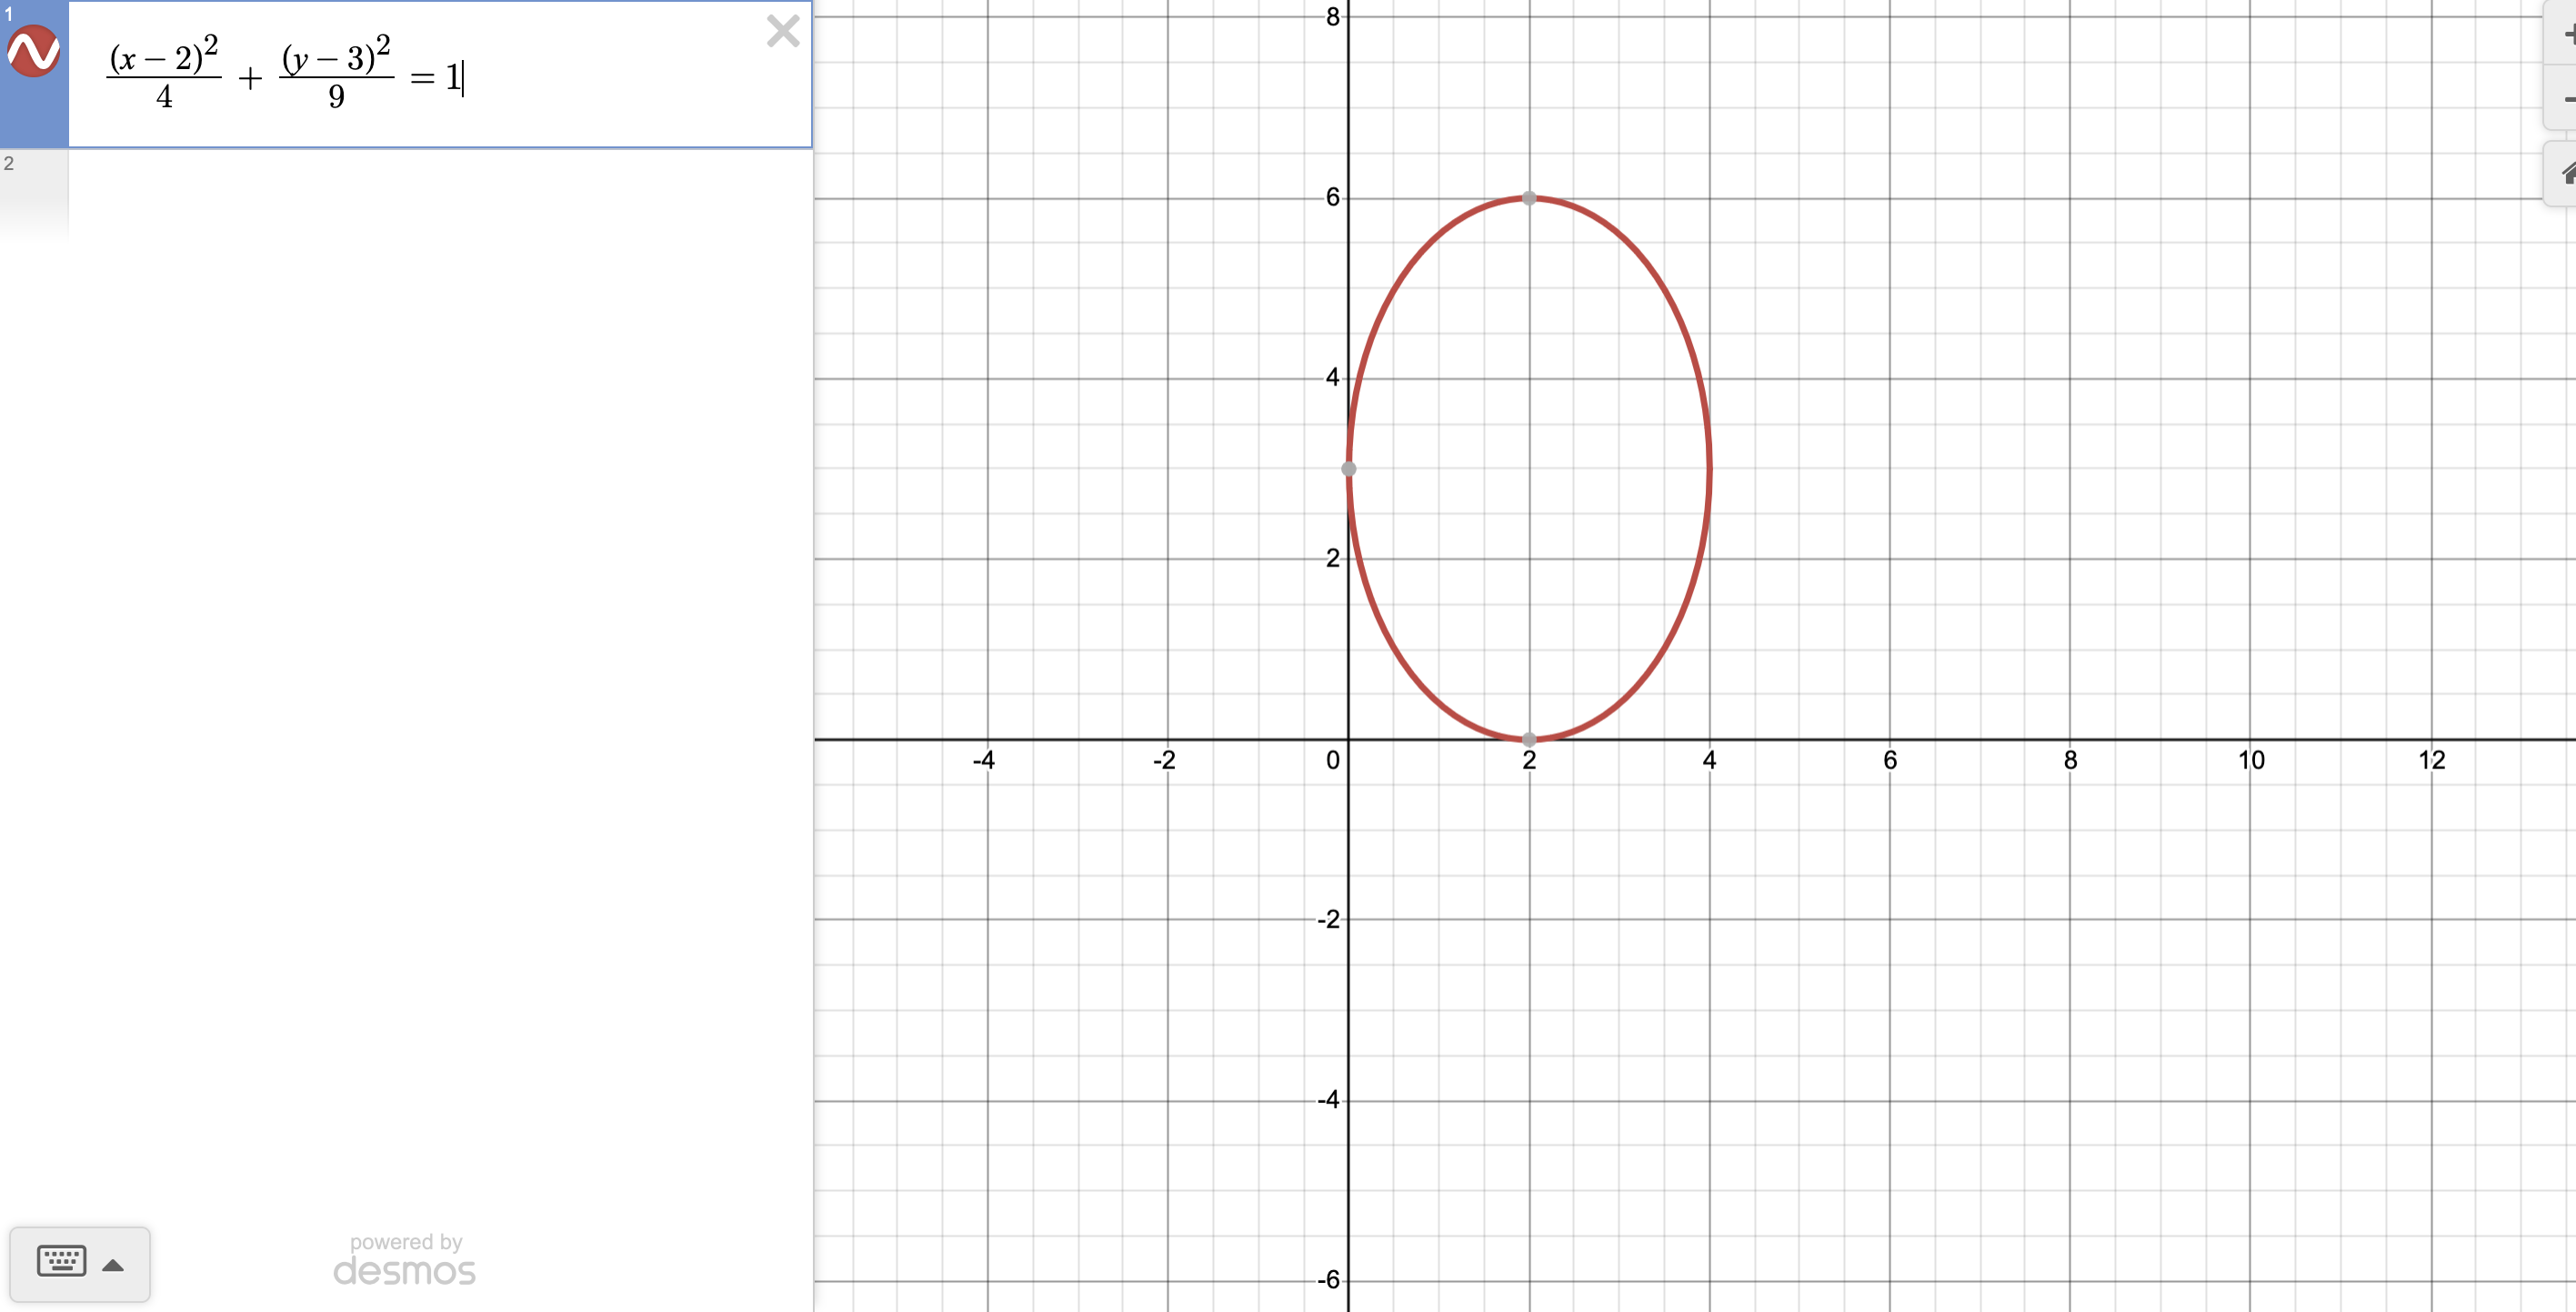
\includegraphics[width = 4in]{41}

\section*{42}
We know that $A=0,B=0$ and $C=1$, meaning the discriminant is $0-0=0$, meaning the conic represented by this equation is a parabola. We need to complete the 
square to turn the equation into one of a parabola:
\[ y^2+14y+16x+33=0 \] \[ y^2+14y+49=-16x-33+49 \] \[ (y+7)^2=-16x+16 \] \[ (y+7)^2=-16(x-1) \]
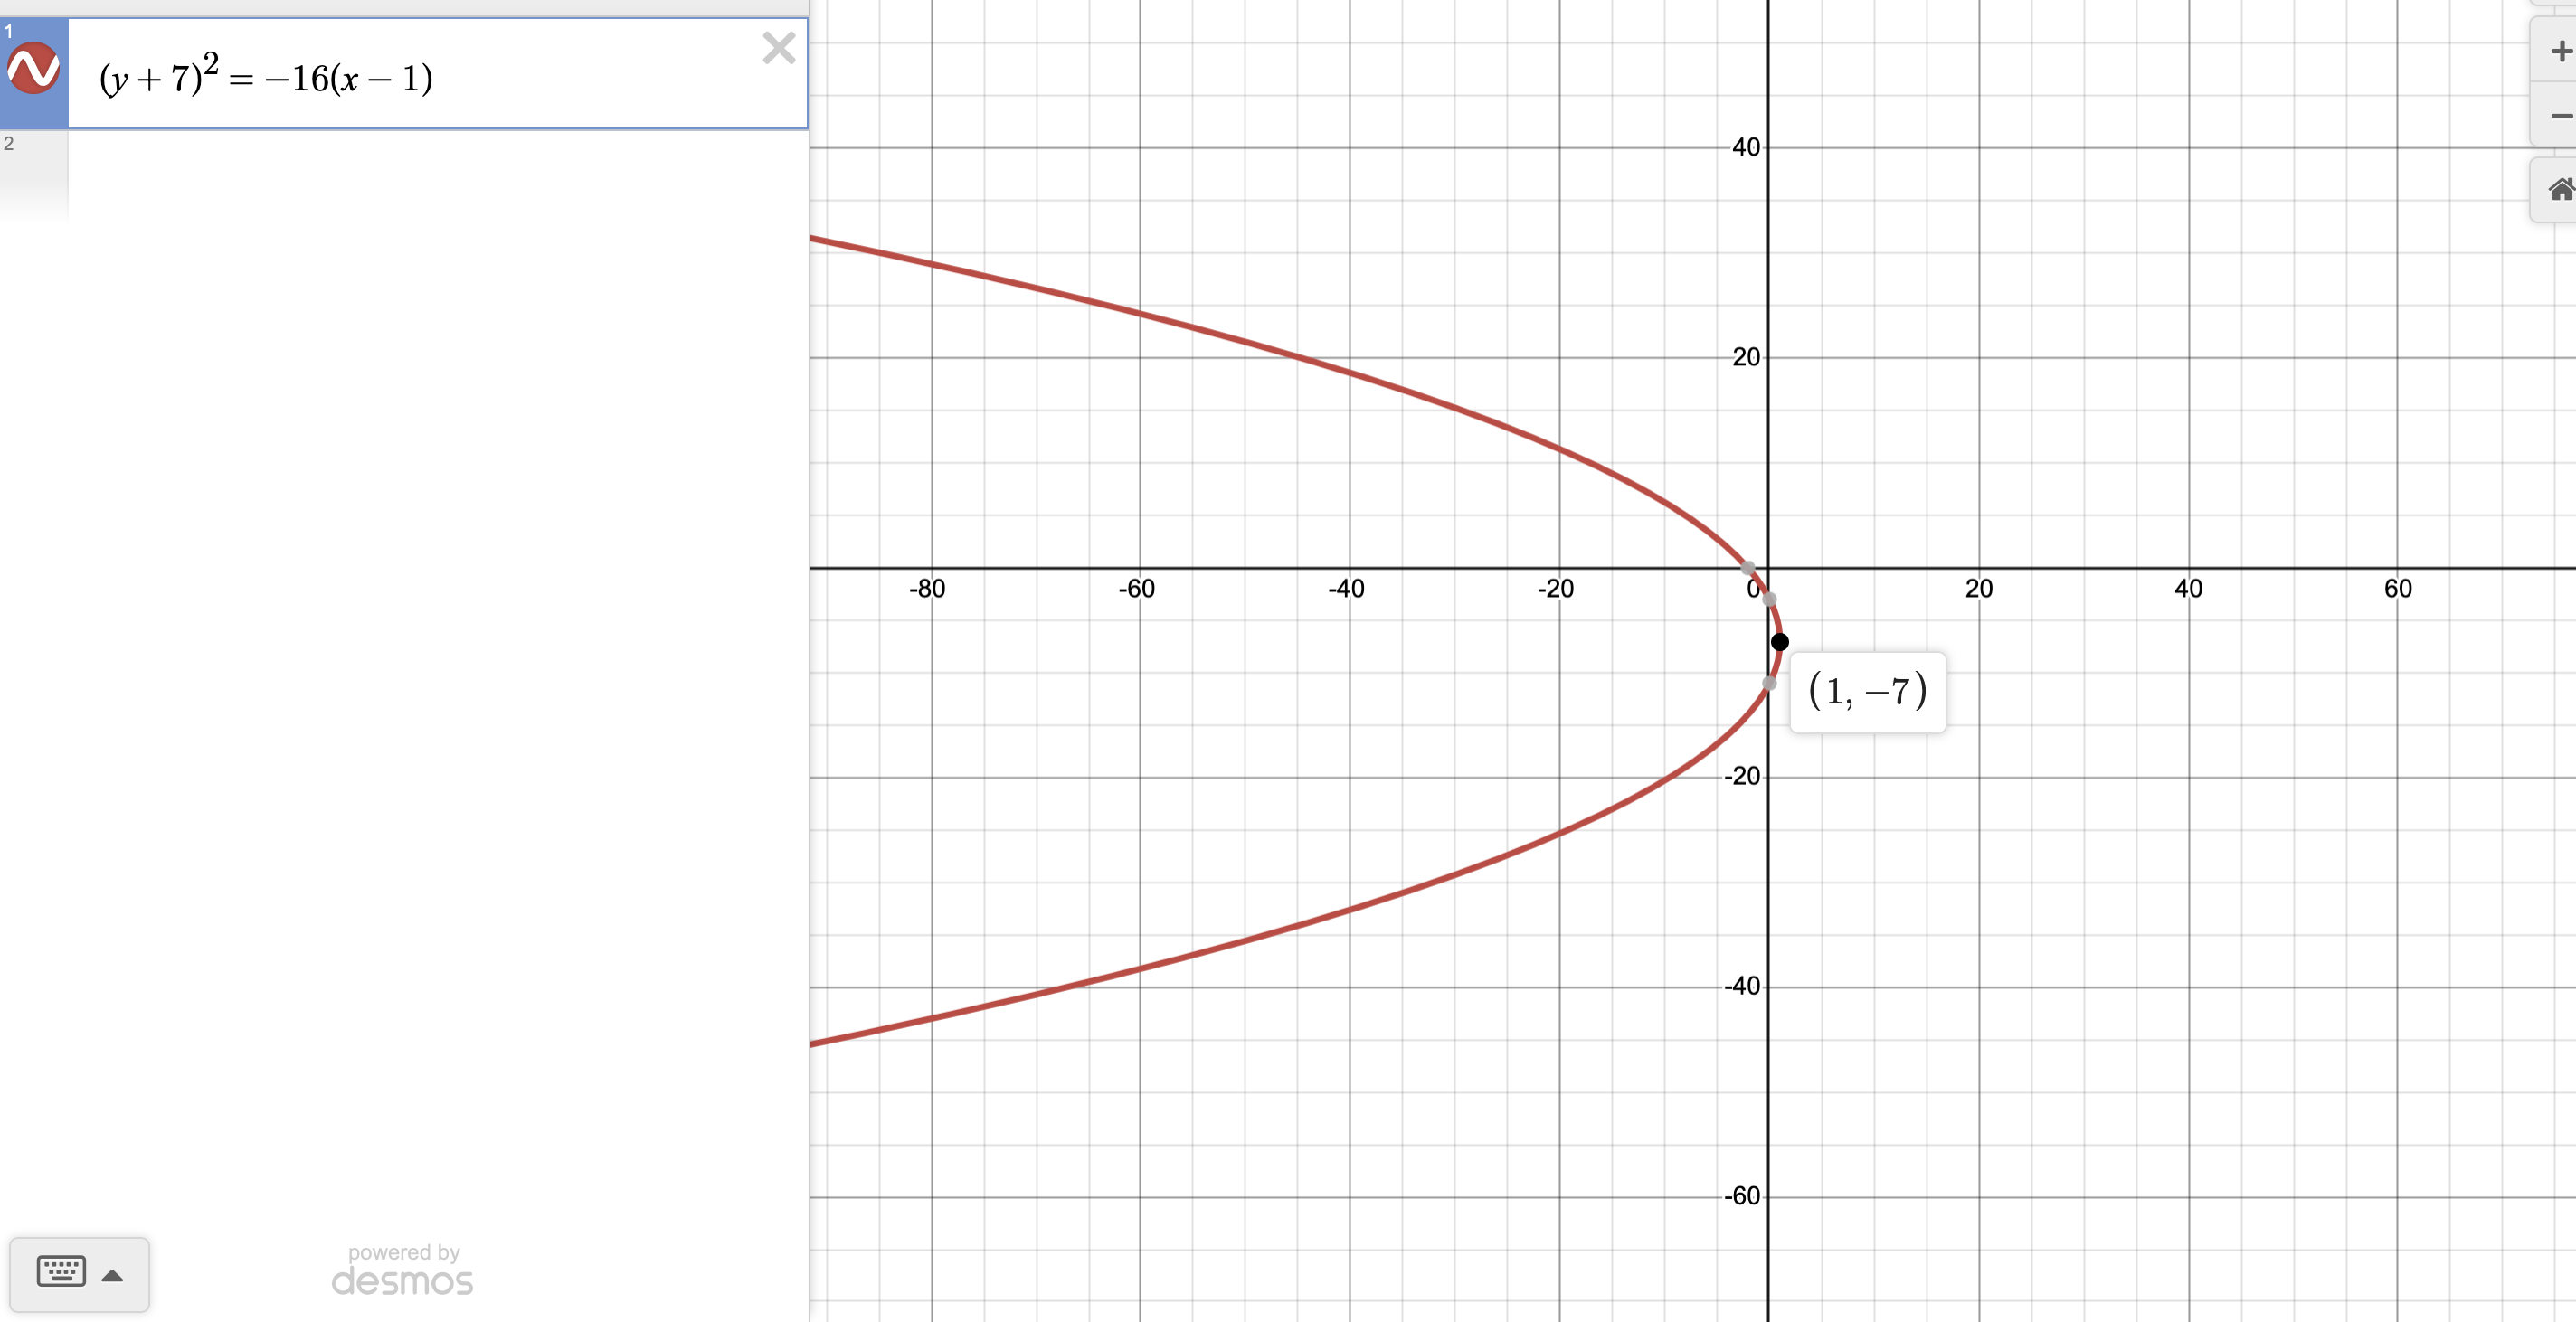
\includegraphics[width = 4in]{42}

\section*{43}
We know that $A=1,B=0$ and $C=1$, meaning the discriminant is $0-4<0$, and because $B=0$ and $A=C$, the conic represented by this equation is a circle. 
We need to complete the square twice to turn the equation into one of a circle:
\[ x^2+y^2+16x-8y+16=0 \]
\[ (x^2+16x+64)+(y^2-8y+16)=64+16-16 \]
\[ (x+8)^2+(y-4)^2=64 \]
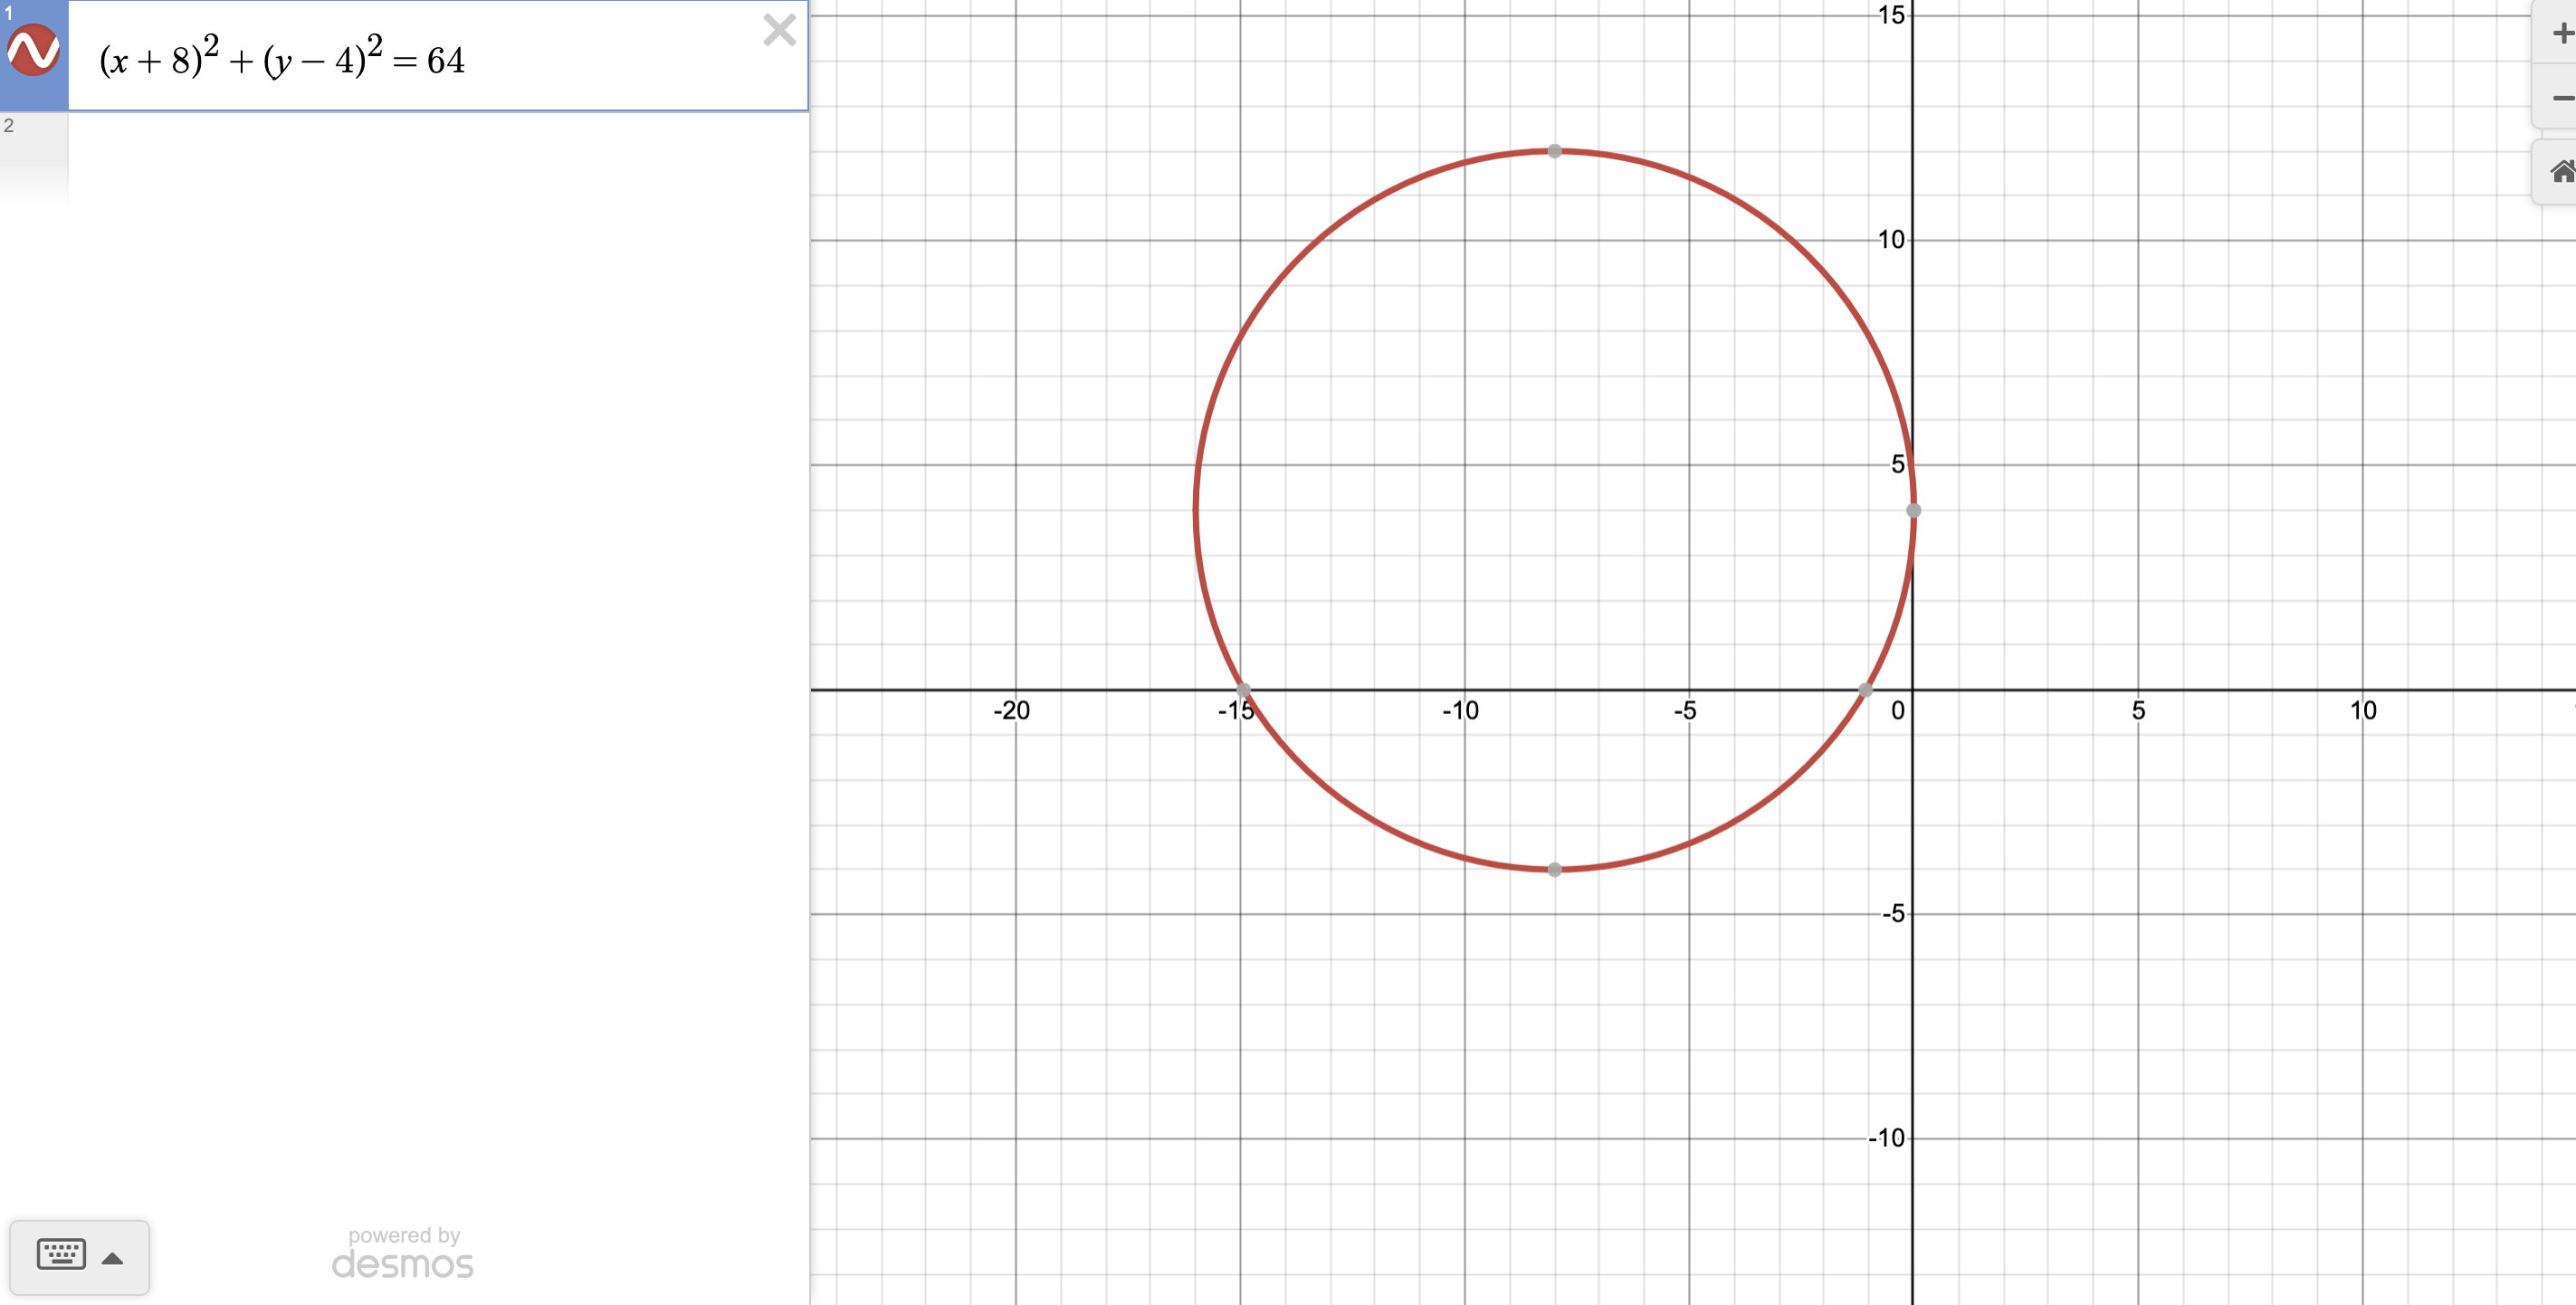
\includegraphics[width = 4in]{43}

\section*{44}
We know that $A=1,B=0$ and $C=-4$, meaning the discriminant is $0-4(-4)=16>0$, meaning the conic represented by this equation is a hyperbola. We need to complete the 
square twice to turn the equation into one of a hyperbola:
\[ x^2-4y^2+8x-24y-24=0 \] \[ (x^2+8x+16)-4(y^2+6y+9)=24+16-36 \]
\[ (x+4)^2-4(y+3)^2=4 \]
\[ \frac{(x+4)^2}{4}-(y+3)^2=1 \]
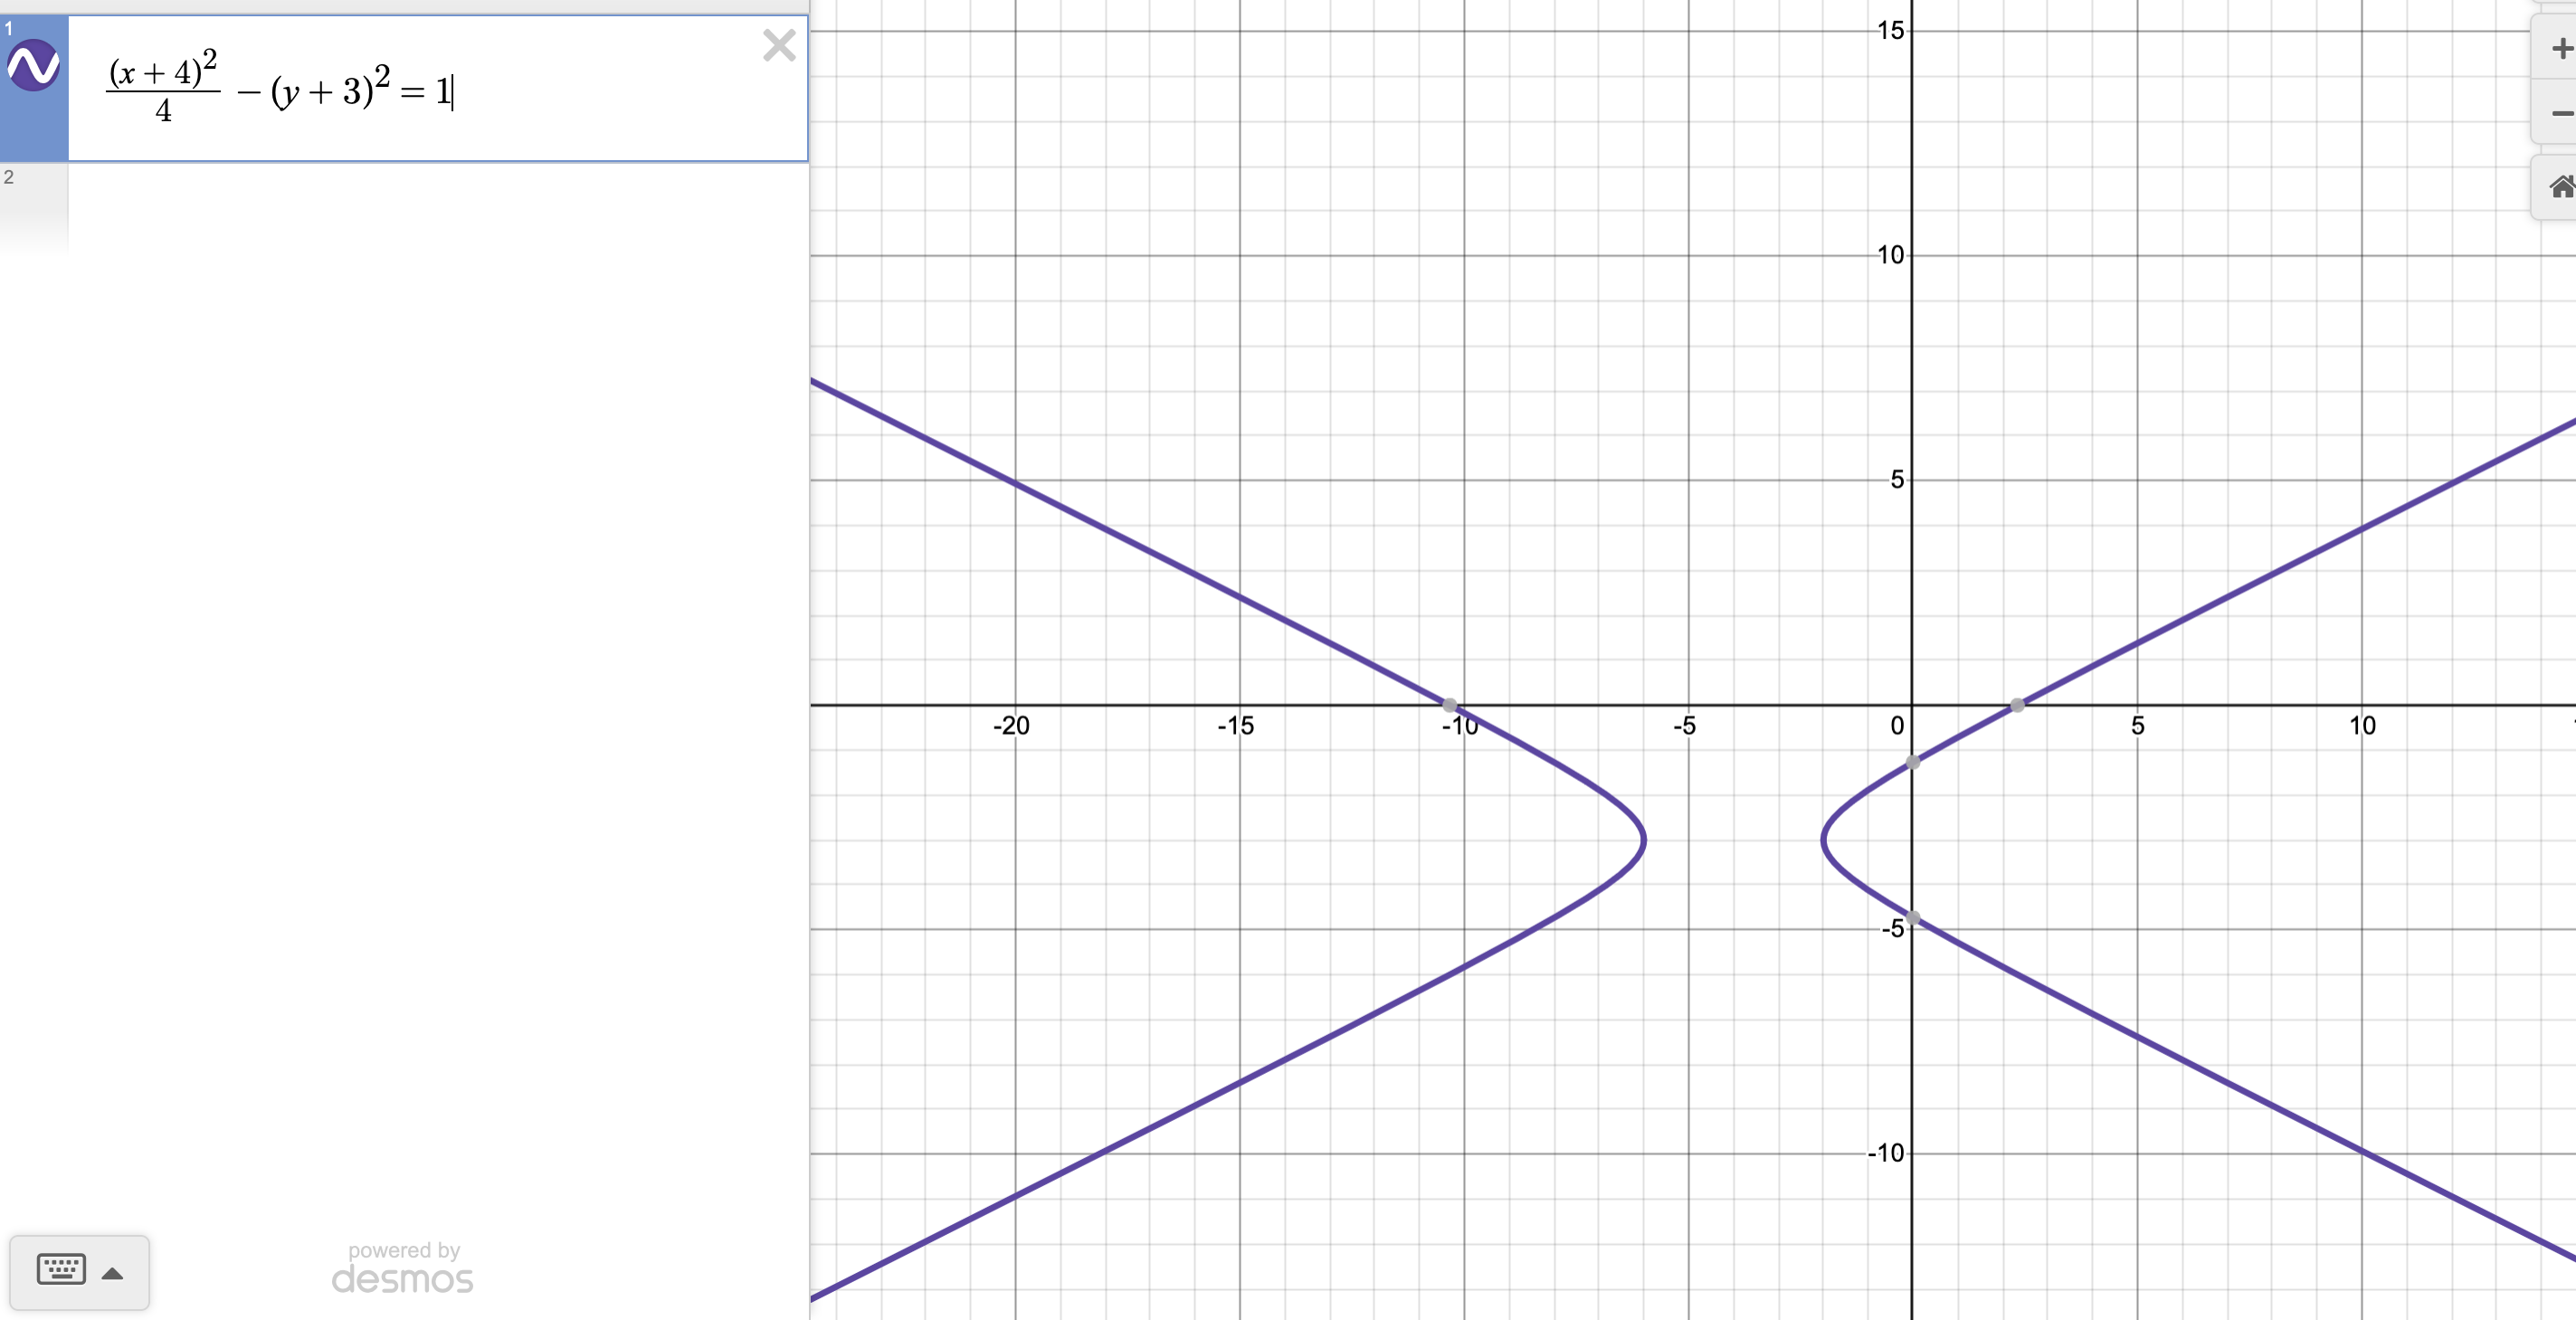
\includegraphics[width = 4in]{44}

\section*{45}
Suppose that we have a general second-degree equation where $B=0$. Then there are two cases: either both $A\ne 0$ and $C\ne 0$, or one of $A$ or $C$ is equal to 0. 
In the first case, we simply complete the square twice in the equation. This will yield us an equation which is either a circle, hyperboala, or an ellipse. Once we have 
that equation, we can determine which one of the preceeding conics that graph is a standard form of. If the latter case, when one of $A$ or $C$ is equal to 0, we 
only complete the square once (for the $A$ or $C$ which is not equal to 0), and we will end up with an equation for a parabola.

\section*{46}
We are given the equation:
\[ y=\frac{a}{x} \] \[ xy-a=0 \] Thus $A=0,B=1$ and $C=0$. Hence the discriminant is $1-4(0)=1>0$, which proves that the graph of this equation is a hyperbola.

\section*{47}
(I was not entirely sure what they meant by asking to write the equation of the asymptotes in terms of $a,b,h,$ and $k$, as one can write the asymptotes with only 
knowledge of $a$ and $b$)\newline
Suppose we are given a hyperbola with a vertical transverse axis and center $(h,k)$. We know that the center is halfway between the two foci. Also, we know that the 
two foci are $(h\pm c,k)$.

\section*{51}
(a): We are given that one transmitter is located 100 yards east and 60 yards south of you, and has a range of 150 yards. The other is located 80 yards west and 70 
yards south of you, and has a range of 100 yards. Suppose that you are located at the origin. Then an equation modeling the points inside of the first circle is
$(x-100)^2+(y+60)^2<150^2$ and an equation modeling the points inside of the second circle is $(x+80)^2+(y+70)^2<100^2$.


(b): \newline 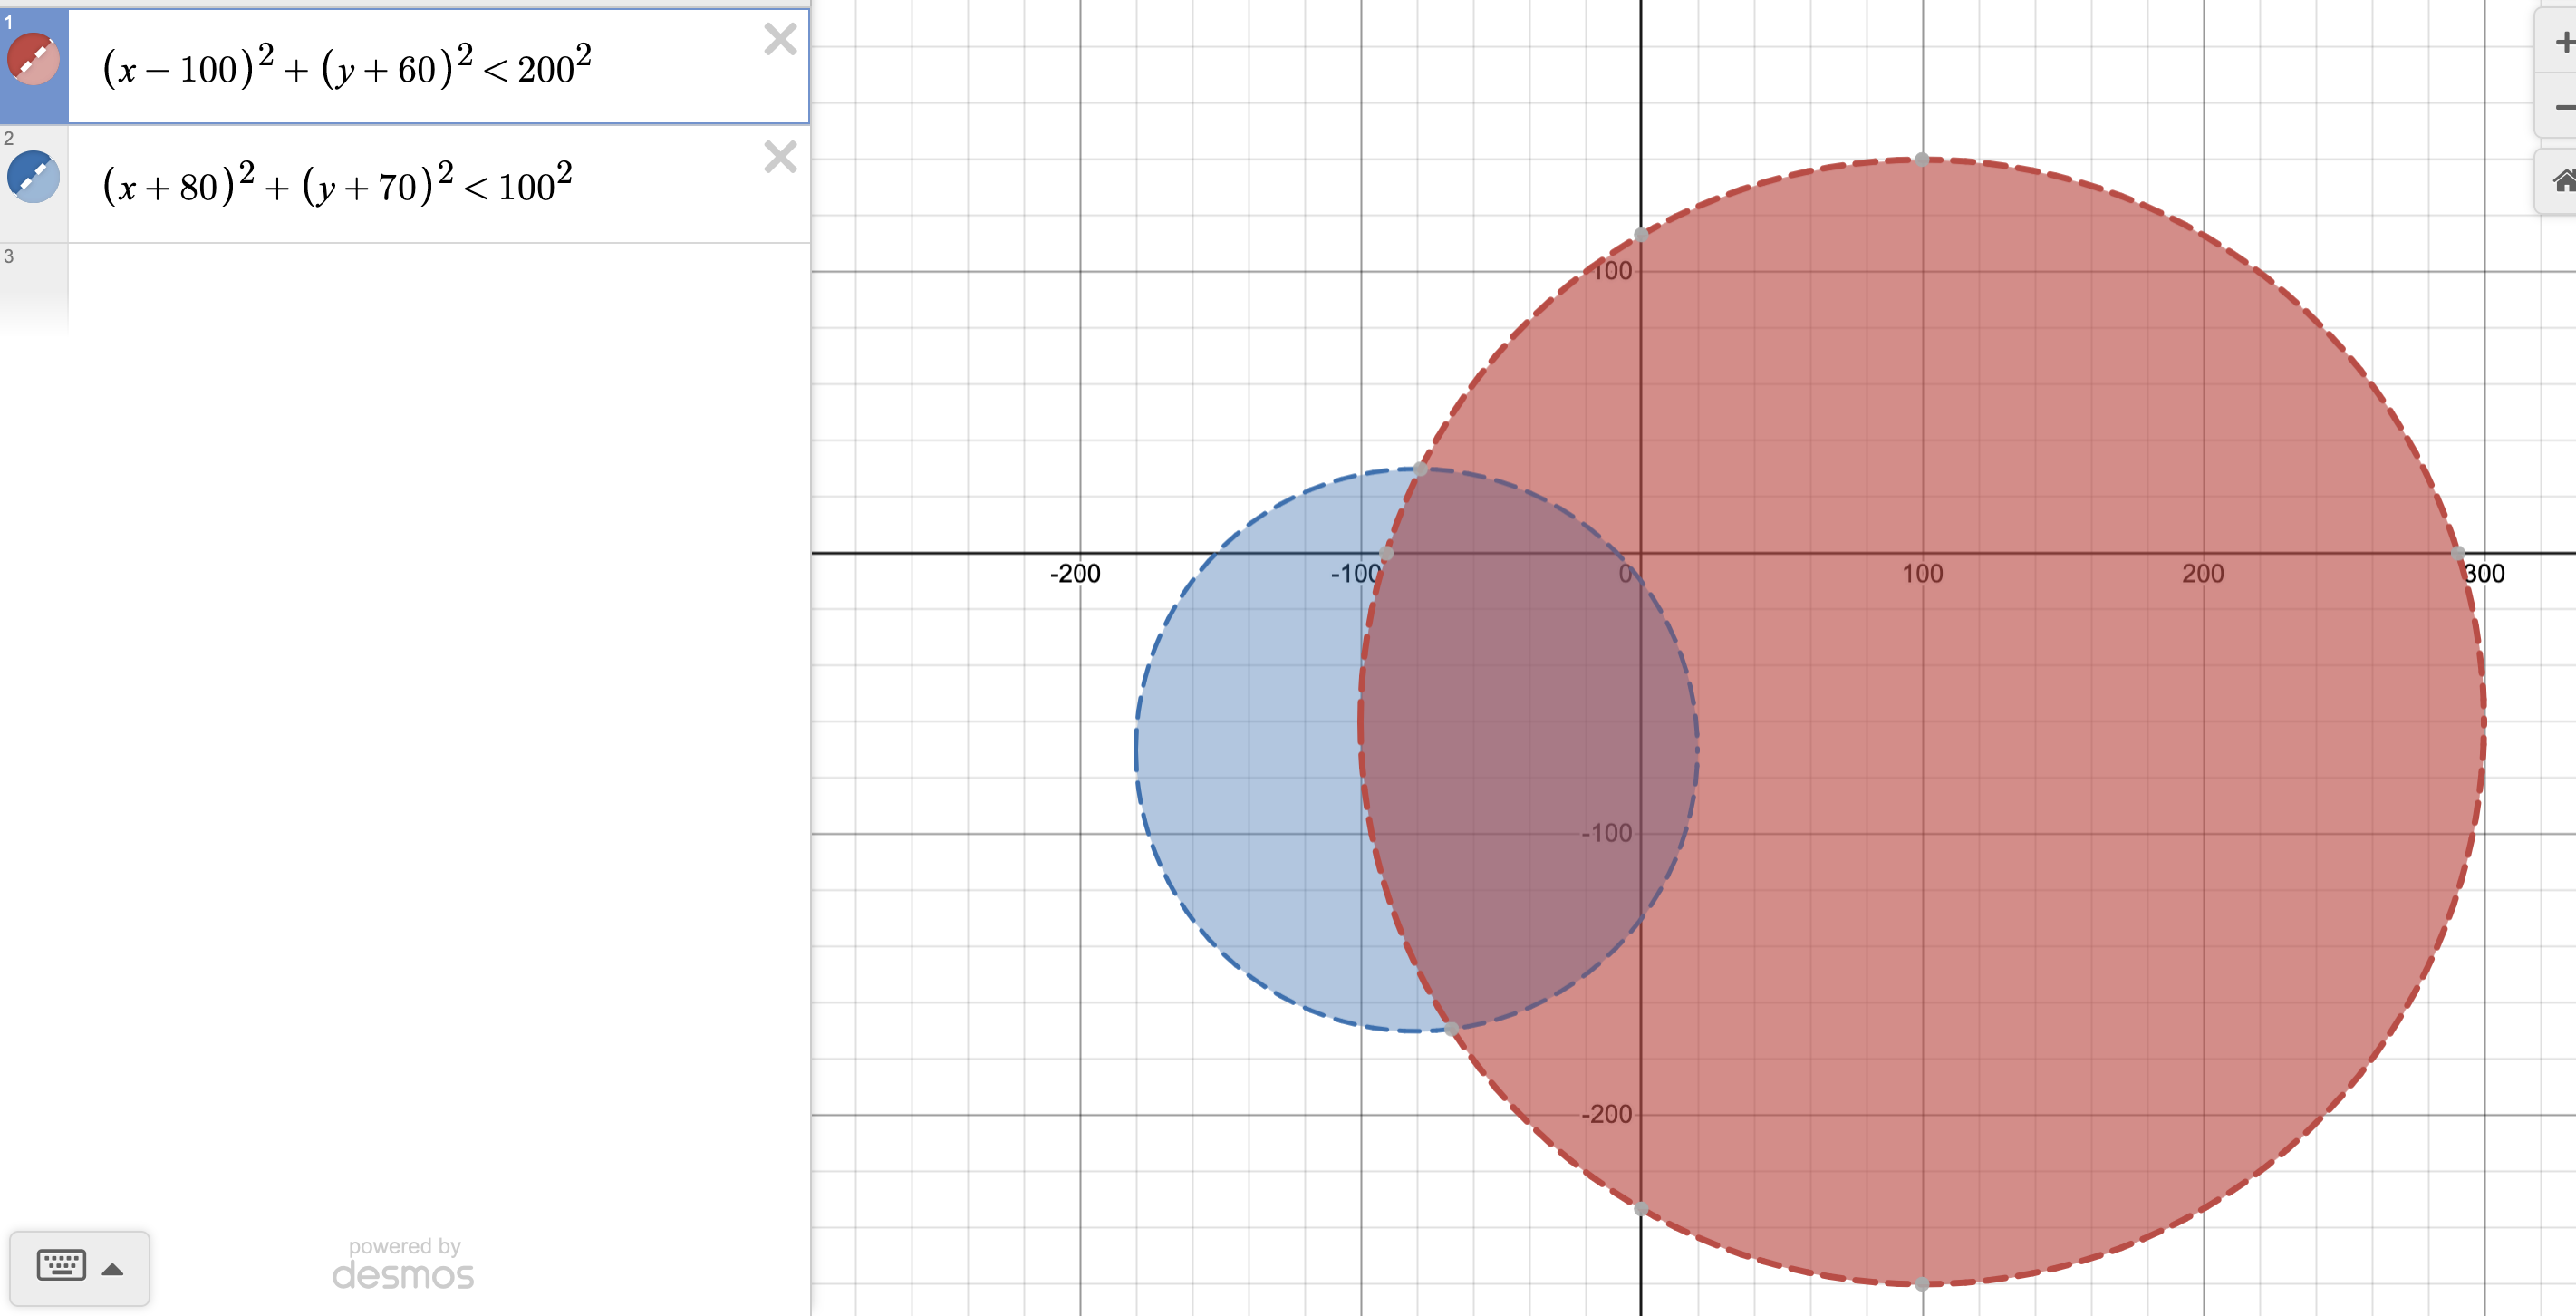
\includegraphics[width = 4in]{51}\newline 
To determine if we are in the first region, we find the distance from the origin to the center. It is $\sqrt{100^2+60^2}\approx 116.6$. Because this is less than $150$, you are 
in range of the first tower. The distance from the origin to the second center is $\sqrt{80^2+70^2}\approx 106.3$. Because this is greater than $100$, you are not in range of the second 
tower. 


(c): In order to answer this question, we first prove the following statement: For any two circles, if the distance between their centers is less than the sum of their two radii, then 
the circles over lap. So suppose that we are given two circles. One is centered at $(h,k)$ with radius $r_1$, and the other is centered at $(a,b)$ with radius $r_2$. We are given 
that the distance between their centers, which is $\sqrt{(h-a)^2+(k-b)^2}$, is less than the sum of their two radii, which is $r_1+r_2$. 
Thus we have:
\[ \textrm{(1)}\sqrt{(h-a)^2+(k-b)^2}<r_1+r_2 \] and \[ \textrm{(2)}\frac{\sqrt{(h-a)^2+(k-b)^2}}{2}<\frac{r_1+r_2}{2} \] 
Now, consider the midpoint of the segment between the two centers of the circles (we will call this segment $S$). It is:
\[ (\frac{h+a}{2},\frac{k+b}{2}) \] The distance between $(h,k)$ and the midpoint is (and we will refer to this distance as $d$)
\[ \sqrt{(h-\frac{h+a}{2})^2+(k-\frac{k+b}{2})^2} \]
\[ =\sqrt{(\frac{h-a}{2})^2+(\frac{k-b}{2})^2} \]
\[ =\sqrt{\frac{(h-a)^2+(k-b)^2}{4}} \]
\[ =\frac{\sqrt{(h-a)^2+(k-b)^2}}{2}<\frac{r_1+r_2}{2}\textrm{ By (2)} \]
Thus we know that $d<\frac{r_1+r_2}{2}$. Then there are two cases: $r_1\ge r_2$ or $r_1<r_2$. In the first case, there are two sub-cases: either $r_2<r_1$ or $r_2=r_1$. 
In the first case, it is obvious that, because $d<\frac{r_1+r_2}{2}$ and $r_2<r_1$, then $d<r_1$. In the second case, we know that 
$d<\frac{r_1+r_2}{2}=\frac{r_1+r_1}{2}=r_1$, that is, $d<r_1$. Thus, in either of these sub-cases, the length between $d$ and $(h,k)$ is less than $r_1$, meaning the midpoint of $S$ is contained 
in the first circle. Now we consider the second case: $r_1<r_2$. Suppose that the midpoint of $S$ was not contained in circle one, that is, $d>r_1$. Consider the distance $d_1$ between 
$(a,b)$ and the midpoint of $S$. Well, it is equal to $d_1$, so it is:
\[ \frac{\sqrt{(h-a)^2+(k-b)^2}}{2}<\frac{r_1+r_2}{2}\textrm{ By (2)} \]
Thus we also know that $d_1<\frac{r_1+r_2}{2}$. But, because $r_1<r_2$, it follows that $d_1<r_2$; hence the midpoint of $S$ is contained in circle two. Now, it was supposed that 
the midpoint of $S$ was not contained in circle two. Hence $d=r_1+m$ for some $m$, and $d_1=r_2-n$, meaning $S=r_1+m+r_2-n$. But it cannot be that $m<n$. For $m$ contains all of the length 
required to get from $r_2$ to the midpoint of $S$, which is $n$. To visualize this, consider the following diagram:\newline
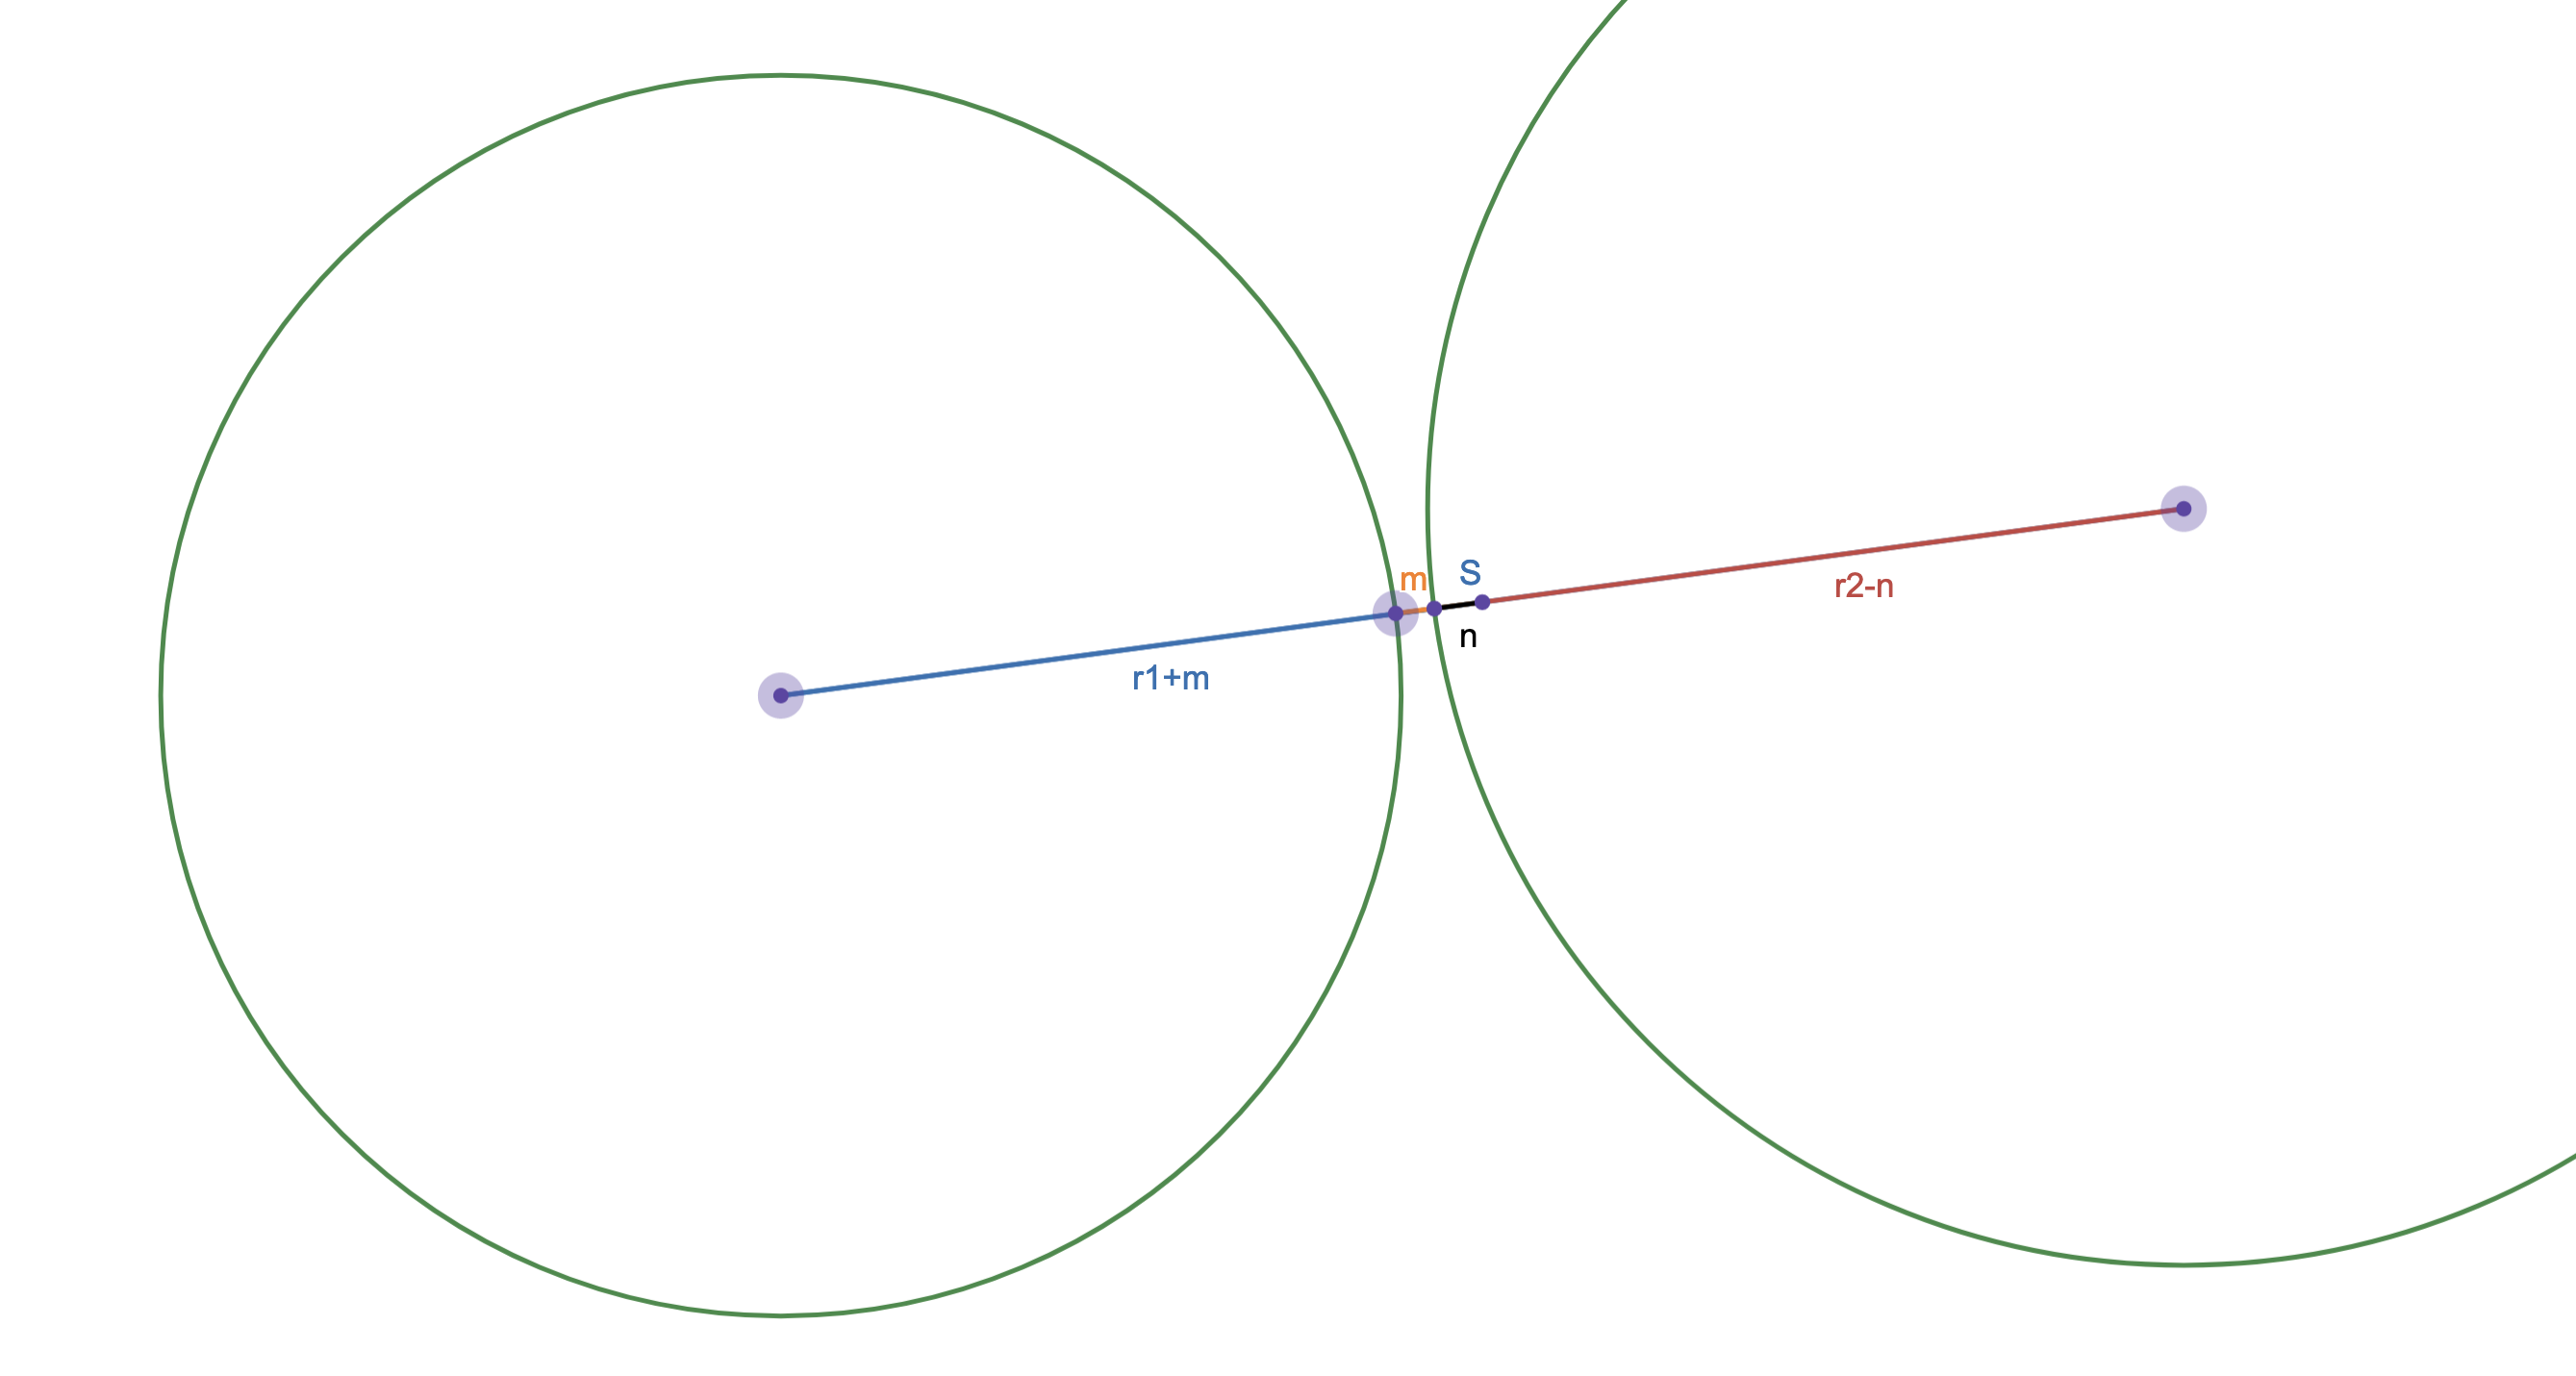
\includegraphics[width = 4in]{51second}\newline
Thus $m\ge n$. To show this more precisely, let $X$ be the point where $S$ intersects circle one, and $Y$ be the point where $S$ intersects circle two. We assume that 
circles one and two do not overlap (if they happen to overlap, then the proof is already done). $m$ is the distance 
between $X$ and the midpoint of $S$ (which we will call $M$), which is at least 0, as we assumed $M$ lied outside of circle one. Because the circles do not overlap, point $X$ 
is either outside of circle two, or intersects it. In either case, the distance between point $X$ and $M$ is greater than or equal to the distance between point $Y$ and $M$ (because the 
segment between $Y$ to $M$ is contained in the segment from $X$ to $M$, as $X$ lies outside of circle two, but $M$ lies inside of circle two); that is, 
$m\ge n$. Hence \[ S=r_1+m+r_2-n\ge r_1+r_2 \] contrary to the assumption that $S<r_1+r_2$. What this means is that 
it cannot be that the midpoint of $S$ lies outside of circle one; hence it does lie in circle one. Similar reasoning with circle two shows that, in any case, the midpoint of $S$ lies in circle two.
Thus we have shown that the midpoint of $S$ lies inside of both circles; hence they overlap.


Knowing this, we need only to show the the sum of the radii of the two circles is less than the distance between their centers. The sum of the radii of the two circles 
is $100+150=250$, while the distance between their centers is:
\[ \sqrt{(-80-100)^2+(-70+60)^2}\approx 180.3 \] meaning the distance between their centers is less than the sum of their radii, and thus they overlap. 
 
\section*{52}
(a): When some plane intersects a conic diagonally, an ellipse is the resulting figure. Thus an ellipse is formed in this situation.


(b): When some plane intersects parallel to the conic, a parabola is formed. Thus a parabola is formed in this situation.

\section*{53}
(a): If the plane perpendicular to the cone's axis passes through the midpoint of the cone, the point of intersection will not longer be a circle, but just a single point.


(b): In this case, the intersection is not a hyperbola when the plane cuts the conic in half. When this occurs, the intersection will be an absolute value function pointing up, and an 
absolute value function pointing downwards.


(c): The intersection will no longer be a parabola when the intersection is only on the nappe which the plane is parallel to. When this occurs, the intersection will form a straight line.

\end{document}
